% main.tex
\documentclass{mathbook} % Use the custom mathbook class
% Title and author
\title{Mathematical Machine Learning}
\author{Yahya \textsc{Saleh}, Tizian \textsc{Wenzel}, Kamal \textsc{Sharma}}

\bibliography{mml}

%%% Added Tizian
\newtheorem{question}{Question}[section]
\newtheorem{prob}{Problem}[section]

\newcommand{\R}{\mathbb{R}}
\newcommand{\N}{\mathbb{N}}
\newcommand{\Ha}{\mathcal{H}}

\newcommand{\ns}{\mathcal H_k (\Omega)}

\newcommand{\tw}[1]{\textcolor{magenta}{TW: #1}}


% \usepackage{showlabels} % use this to show labels of formula!



\begin{document}


\frontmatter % Front matter (title page, table of contents, etc.)

\maketitle % Title page

\tableofcontents % Table of contents
\pagenumbering{arabic} % Change page numbering style to Arabic numbers
% Include Chapters from the 'Chapters' folder
\include{Chapters/Chapter1}
\include{Chapters/Chapter2}
% Chapter 1
% !TeX spellcheck = en_US 
\chapter{Neural networks} % Main chapter title

\label{Chapter3} % For referencing the chapter elsewhere, use \ref{Chapter1} 
\setcounter{chapter}{3}
%\setcounter{section}{0}
In the \nameref{Chapter1} chapter, we breifly talked about a neural network which can be used 
to recognize hand-written digits. The neural network takes an image of a hand-written digit as 
an input and predicts a number which corresponds to the digit as an output. In this chapter, 
we will delve deeper into the architecture of neural networks and try to answer the following questions:
\begin{enumerate}
    \item What is the motivation behind using neural networks ?
    \item What is the idea behind the structure (neurons, input layer, hidden layers, output layer) 
    of neural networks ?
    \item Why do we need an activation function and a loss function ?
    \item How to train a neural networks ?
    \item What are learning algorithms ?
    \item Why certain neural networks can approximate any continuous function defined on a compact set ?
\end{enumerate}
Recognition of handwritten digits is a classic problem for introducing the topic of neural networks. Therefore 
we will use this problem as an example to introduce various concepts related to neural networks.
% \begin{figure}[htbp]
%     \centering
%     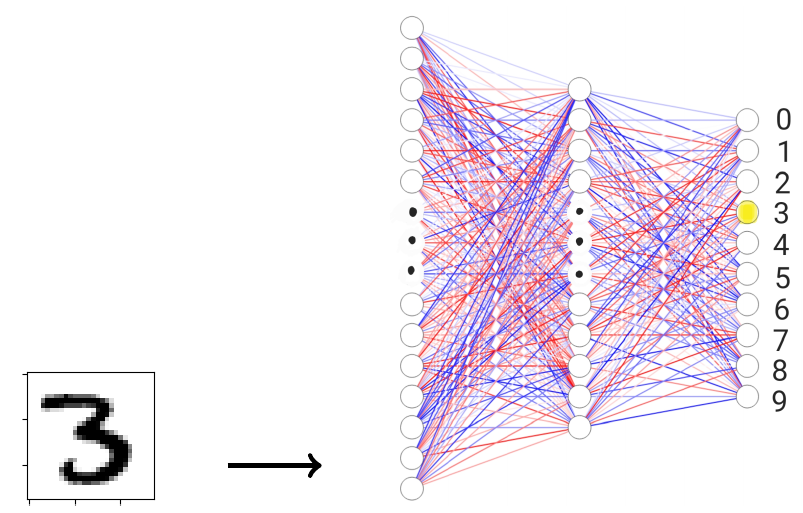
\includegraphics[width=0.8\textwidth]{Figures/ff_net.png}
%     \caption{A feed-forward neural network which can recognize hand-written digits.}
%     \label{fig:ffnet}
% \end{figure}   
%%%%%%%%%%%%%%%% Handwritten digit recog %%%%%%%%%
\section{Handwritten digit recognition}
Most people can easily recognize the handwritten digits shown in figure \ref{fig:my_digits}. Even if these digits were written 
in a different manner (for example refer figure \ref{fig:my_threes} ), one would still be able to recognize them. 
\begin{figure}[htbp]
    \centering
    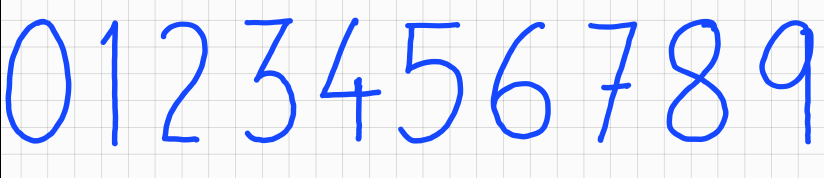
\includegraphics[width=.6\textwidth]{Figures/digits.png}
    \caption{One of the ways of writing digits from $1$ to $9$.}
    \label{fig:my_digits}
\end{figure} 
\begin{figure}[htbp]
    \centering
    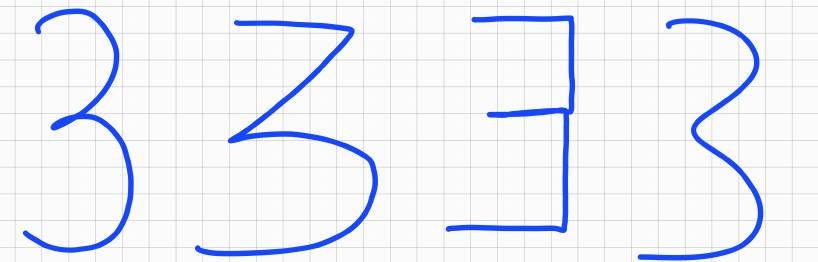
\includegraphics[width=.3\textwidth]{Figures/three_digit.png}
    \caption{Different ways of writing the digit $3$.}
    \label{fig:my_threes}
\end{figure} This is due to the fact that our visual cortex has evolved over millions of years and therefore is magnificently 
adapted to understand the visual world. The problem of recognizing hand-written digits is so trivial 
for our brains that we don't have to put an effort to recognize digits. But this task will immediately 
start to look complicated when one tries to write a computer program which can recognize hand-wriiten 
digits. 
Let us try to write a program for this task. We can start by coverting the digits into a pixel 
image ($28 \times 28$ for example) and assign each a value from $0$ to $1$ based upon the level of darkness
of each pixel (figure \ref{fig:pix7}). This can serve as an input to our program. 
\begin{figure}[htbp]
    \centering
    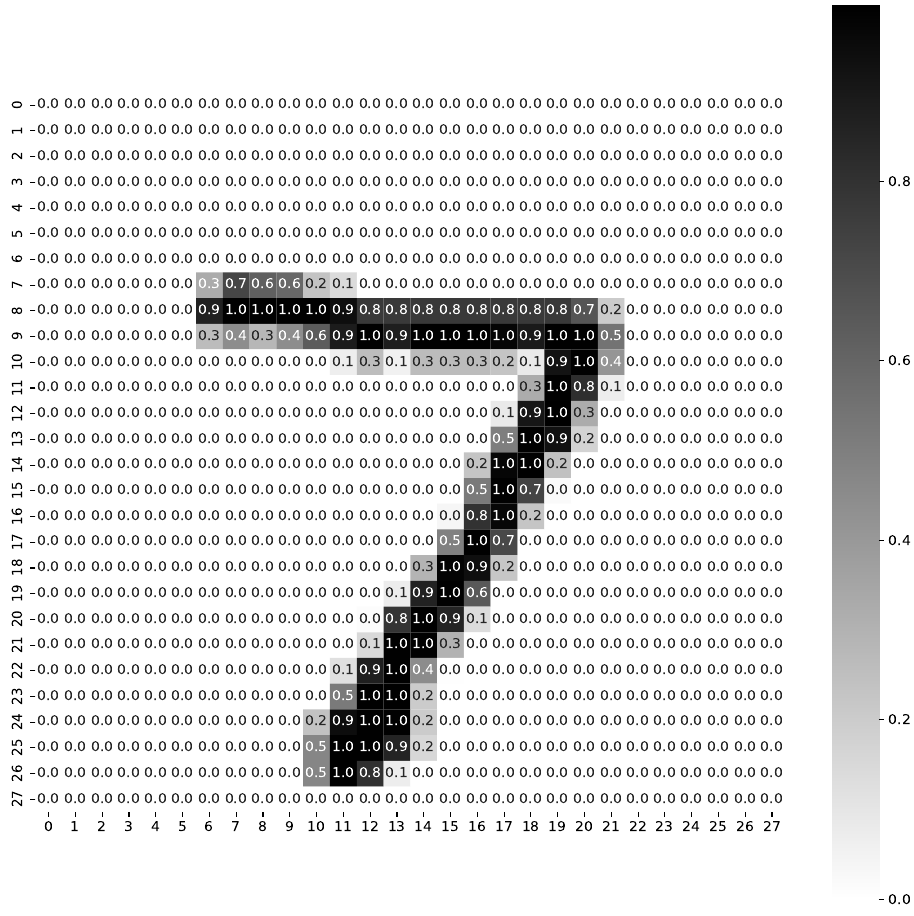
\includegraphics[width=.35\textwidth]{Figures/pixel_image_7.png}
    \caption{A $28 \times 28$ pixel image of digit $7$. Each pixel is assigned a value from $0$ to $1$.}
    \label{fig:pix7}
\end{figure} 
We can identify distinct features of each digit and write code which looks for these features in the input image. 
Our program will therefore contain a lot of \emph{if} statements and \emph{for} loops to identify such features 
but more importantly will contain thousands of line of code to handle exceptions which arise from the fact that 
each digit can be written in a slightly different manner. It turns out it is very difficult to express algorithmically 
the intuitions we have to recognize digits. Soon we will realize the complexity of this task. What if we could write a 
program (for such fuzzy and difficult to-reason-about problems) that mimics the structure of our brain ?  
% \begin{figure}
%     \centering
%     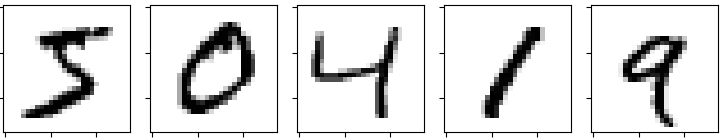
\includegraphics[width=.6\textwidth]{Figures/mnist_digits.png}
%     \caption{A sample of hand-written digits taken from MNIST dataset.}
%     \label{fig:mnist}
% \end{figure} 
% \begin{figure}
%     \centering
%     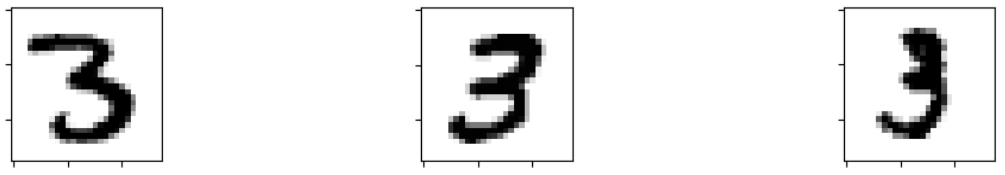
\includegraphics[width=.7\textwidth]{Figures/mnist_3s.png}
%     \caption{A sample of hand-written digit $3$ taken from MNIST dataset.}
%     \label{fig:mnist_3s}
% \end{figure} 
%%%%%%%%%%%%%%%% Intro to NN %%%%%%%%%%%%%
\section{Introduction to neural networks}
Neural networks tackles this problem in a different way. The construction of neural network
is inspired by the structure of our brain. 
\begin{figure}[htbp]
    \centering
    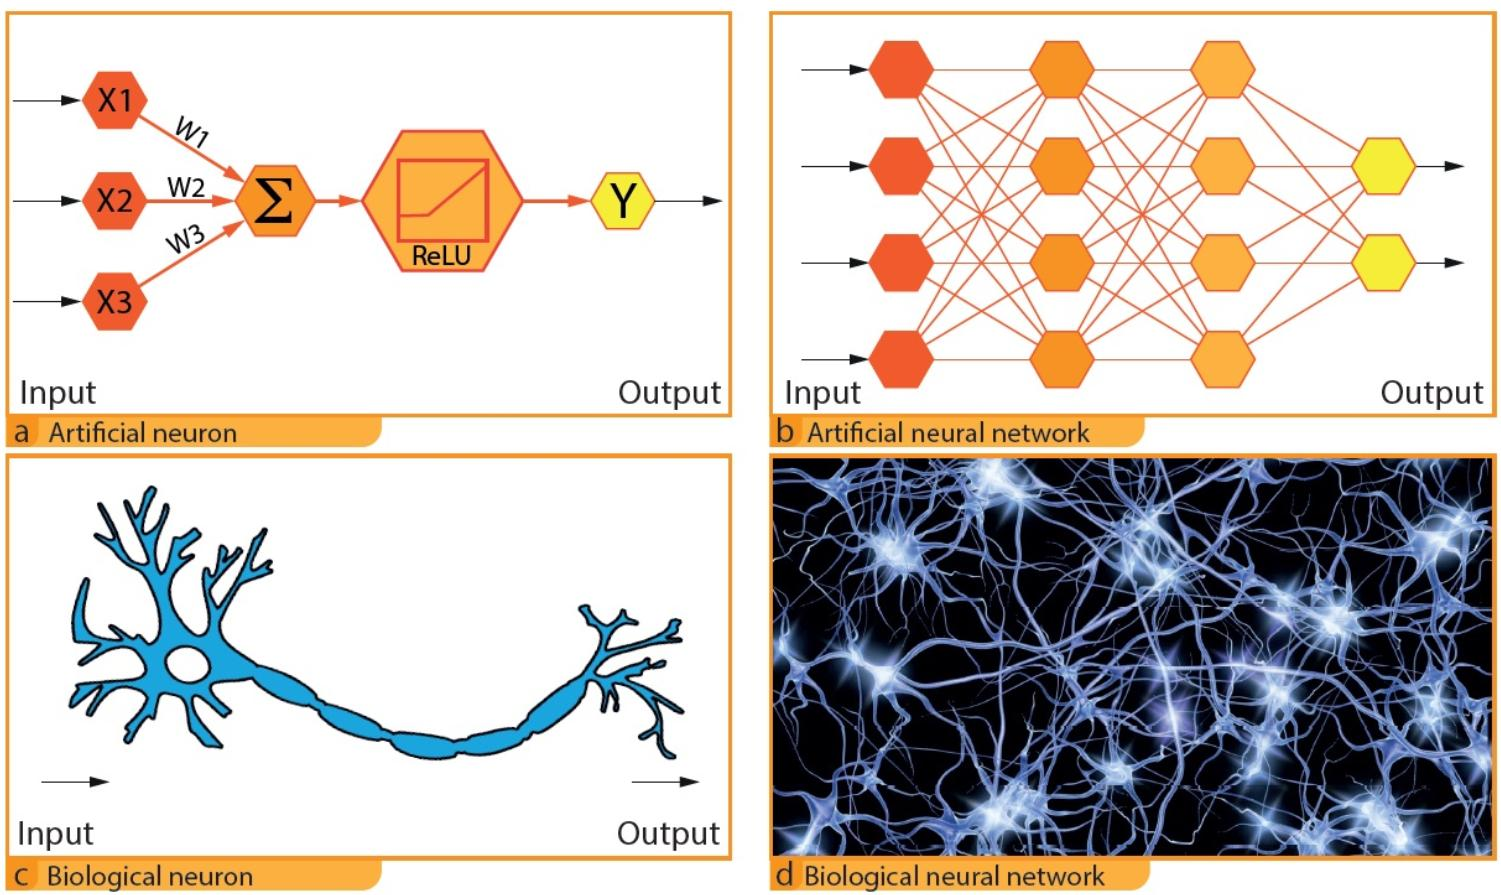
\includegraphics[width=.5\textwidth]{Figures/artificial_vs_normal_neurons.png}
    \caption{Similarity between the structure of artificial and biological neuron.}
    \label{fig:bio_neu}
\end{figure} 
The idea is to take a large number of handwritten digits together with labels and develop a system 
which can learn from these examples just like we learn. We leave it to the system to automatically infer rules 
from these examples and classify hand-written digits. 
\begin{figure}[htbp]
    \centering
    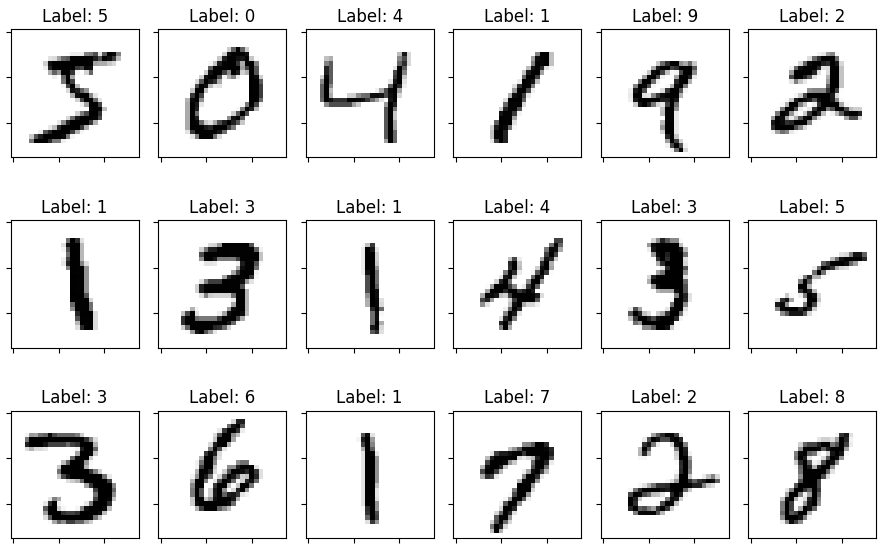
\includegraphics[width=.5\textwidth]{Figures/training_examples_mnist.png}
    \caption{Some training examples from MNIST dataset.}
    \label{fig:train_MNIST}
\end{figure} 

A neural network takes an input and given an output. Figure \ref{fig:ff_net} shows a pictorial representation of
a neural network which can be used to classify handwritten digits. It has layers (input, hidden, output) which consist of 
artificial neurons. The neurons are connected. Each neuron stores a value (for example from $0$ to $1$ in 
our case of handwritten digit recognition). 
\begin{figure}[htbp]
    \centering
    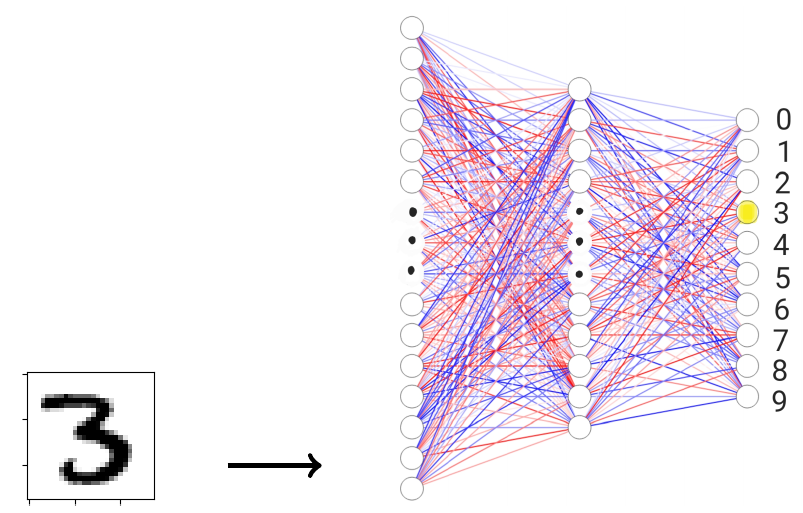
\includegraphics[width=.8\textwidth]{Figures/ff_net.png}
    \caption{A neural network to classify handwritten digits}
    \label{fig:ff_net}
\end{figure} 
A neuron takes multiple inputs (say $a_1, a_2,....,a_n$) and gives the output $\sigma(\sum_{i =1}^n a_i w_i + b)$ where $\sigma$ is
called an activation function. The inputs are multiplied by weights, $w_i$ and added to bias, $b$ before passing through the activation funciton.
The choice of activation function depends on the type of problem one is trying to solve. For example, for hand-written digit recognition one could use sigmoid/logistic function
as an activation function. 
\begin{figure}[htbp]
    \centering
    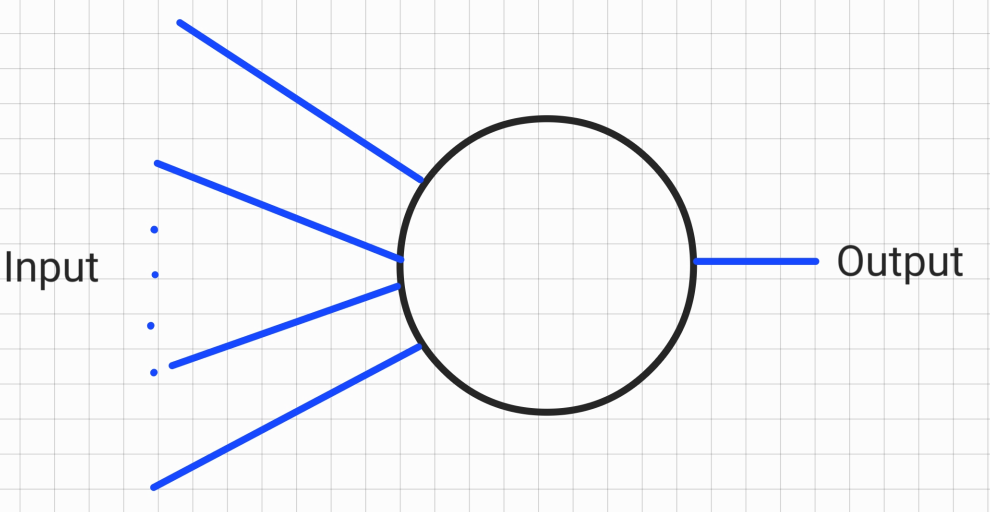
\includegraphics[width=.4\textwidth]{Figures/neuron.png}
    \caption{Pictorial representation of an artificial neuron. Elaborate}
    \label{fig:neuron}
\end{figure} 
\begin{figure}[htbp]
    \centering
    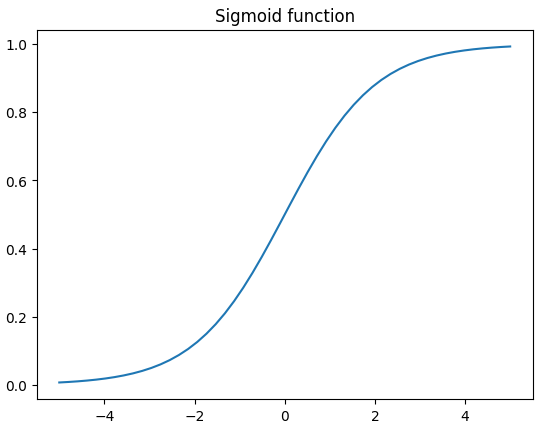
\includegraphics[width=.4\textwidth]{Figures/sigmoid.png}
    \caption{A sigmoid/logistic activation function, $\sigma (z) = \frac{1}{1+ e^{-z}}$}
    \label{fig:sig}
\end{figure} 

Mathematically speaking, a neural network is simply a function that takes an input which passes through
its layers (made up of neurons which are mathematical functions) and results in an output. The neural 
network shown in figure \ref{fig:ff_net} has $784$ neurons in the input layer (containing data from a $28 \times 28$ pixel image), $15$
neurons in the hidden layer and $10$ neurons in the output layer. Each neuron in the output layer corresponds to a digit from $0$ to $9$; if
the input image is of digit $3$, only the fourth neuron in the outplayer will light up (output is close to $1$) while the rest will remain dormant (outputs are close to $0$).
Such neural networks are called feed-forward neural networks. When we look at the architecture of a neural network, many questions can 
come to our mind, for example, 
\begin{enumerate}
    \item Why the network has this structure (i.e. layers with neurons) ?
    \item What is the purpose of using an activation function ?
    \item How does a neural network able to recognize hand-written digits ?
\end{enumerate} 
It is not clear why this appraoch of using neural networks even works. Even if we assume that this approach works, another question arises,
which is, how do we get the weights, $w_i$ and biases $b_i$ of the network ? The answer to this question
comes from a key ability of neural networks which is \emph{learning}.
%%%%%%%%%%%%%%%% Learning from data %%%%%%%%%%%
\subsection{Learning from data}
Learning is the process of obtaining suitable weights and biases such that a neural network can perform
the desired task. There are several steps involved in learning. First step is to assign random values to 
weights and biases of the network and show the network some training examples. In the case of handwritten digit recognition
we use MNIST dataset. Since the network is initialized with random weights and biases it will wrongly classify handwritten digits. 
\begin{figure}[htbp]
    \centering
    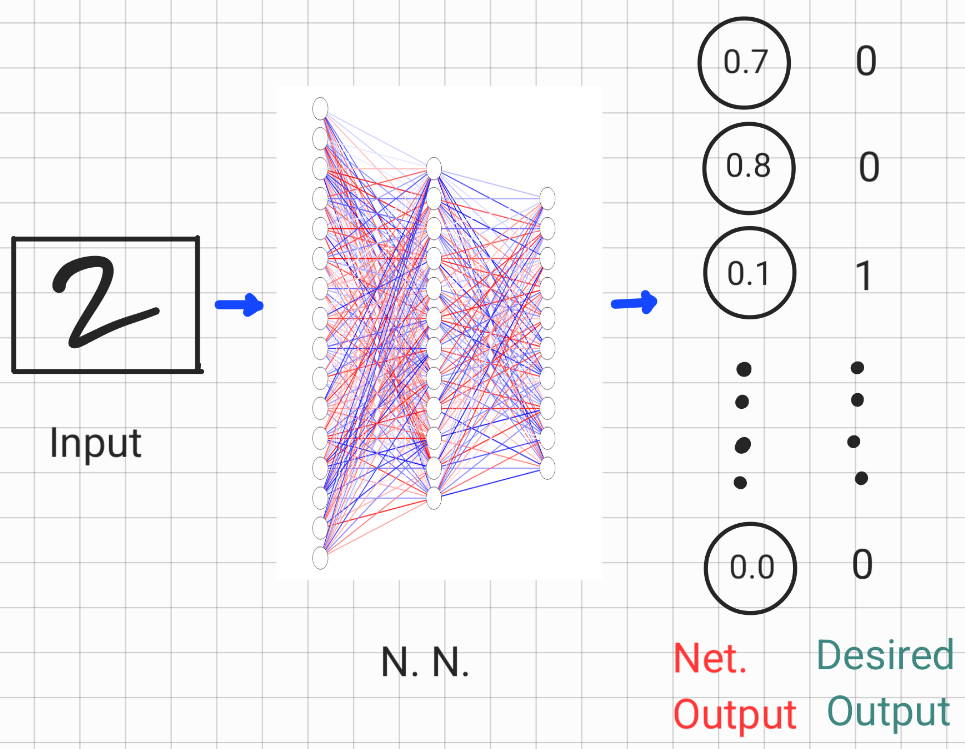
\includegraphics[width=.4\textwidth]{Figures/rand_inp.png}
    \caption{Results from a randomaly initialized neural network and how it compares to the desired output for a training example}
    \label{fig:randinp}
\end{figure} 
Next step is to tell the network to update its weights and biases in order to reduce the classfication error. This is done by introducing a 
cost/loss function which can quantify the classification error. We use a quadratic loss function, 
$$C(w,b) = \frac{1}{N} \sum_x {\|y(x) - a\|}^2$$
where $N$ denotes the number of training examples, $y(x)$ is the desired output corresponding to training example $x$, and 
$a$ is the neural network output. Our aim is to find $w,b$ such that the loss is minimum. The problem of learning from training data thus translates into
solving an optimization problem. But this process raises another set of questions,
\begin{enumerate}
    \item Which optimization algorithm to choose for minimizing the cost function?
    \item How to define a suitable loss function ?
    \item Does a global minimum exists for a chosed loss function ?
\end{enumerate}
The answer these questions and the questions that we raised earlier we will have to first understand the origins of neural networks.
%%%%%%%%%%%%%% Origins of NN %%%%%%%%%%%%%%
\subsection{Origins of neural networks}
The artificial neurons we introduced earlier are called sigmoid neurons. In order to understand 
why sigmoid neurons are defined the way they are, we need to first understand another artificial 
neuron called perceptron. Perceptrons were developed in the $1950$s and $1960$s. Unlike sigmoid neurons 
whose inputs, $x_i \in \mathbb{R}$, a perceptrons can take only binary inputs and produce a binary output.
The mathematical model of a perceptron is,
\begin{equation*}
    \text{output} = 
     \begin{cases}
       0 &\quad \text{if} \ \ \sum_i w_i x_i \leq \ \text{threshold} \\
       1 &\quad  \text{if} \ \ \sum_i w_i x_i > \ \text{threshold} 
     \end{cases}
\end{equation*}
where $x_i$ are the inputs and $w_i$ are the weights. The output is $1$ if $\sum_i w_i x_i$ exceeds a threshold 
value otherwise the output is $0$. Perceptrons can be used as a device to make simple decisions by weighing up evidence. 
The following example illustrates how perceptrons can be used to make a decision.
\begin{boxedexample}
    Suppose a rock band is coming to perform in your city. You like rock music, and are trying to 
    decide whether or not to go to this event. You can make the decision by weighing up three factors:
   \begin{enumerate}
    \item Is the event nearby ?
    \item Are your friends accompanying you ?
    \item Is the weather good ?
   \end{enumerate}
   We can assign binary variables $x_1, x_2$ and $x_3$ to these three factors. For example, if the event is nearby we would
   have $x_1 =1$ but if it is far away we would have $x_1 = 0$. Similarly, if your friends are accompanying you, $x_2 =1$ otherwise $x_2 =0$.
   If the weather is good, $x_1 =0$ and if the weather is bad, $x_3 =0$. Now suppose, you absolutely love rock music and it doesn't really 
   matter to you if your friends can accompany you or if the event is nearby but you really loathe bad weather and you won't go if the
   weather is bad. You can use perceptrons to model this kind of decision-making. One way is to choose, $w_3 = 6$ for the weather and
   $w_1 =2, w_2 =2$ for other conditions. The larger value of $w_3$ in comparison to $w_1$ and $w_2$ suggests that weather matters to you a lot. 
   Finally, suppose you choose a thresold value of $5$ for the perceptron. With these choices, the perceptron mimics the desired 
   decision-making model, outputting $1$ whenever the weather is good, and $0$ whenever the weather is bad. By choosing different values for 
   weights and the thresold, we can get different models of decision making. 
\end{boxedexample}
It is obvious that the perceptron isn't a complete model of human descision-making. But it is plausible that if we use more layers in the network
with more number of perceptrons, the network could make more complex descisions:
\begin{figure}[htbp]
    \centering
    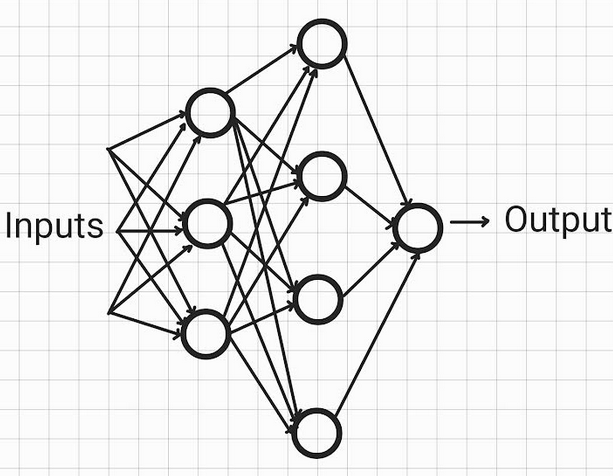
\includegraphics[width=.4\textwidth]{Figures/perceptron_network.png}
    \caption{A network built out of perceptrons.}
    \label{fig:percep_net}
\end{figure} 
We can write the mathematical model of a perceptron in a way familiar to us, 
\begin{equation*}
    \text{output} = 
     \begin{cases}
       0 &\quad \text{if} \ \ \sum_i w_i x_i + b \leq 0 \\
       1 &\quad  \text{if} \ \ \sum_i w_i x_i + b > 0 
     \end{cases}
\end{equation*}
where perceptron's bias, $b \equiv -$threshold. We have seen that a network of perceptrons can be used as 
a method for weighing evidence to make decisions. We can also use perceptrons to compute the elementary logical functions such as
AND, OR, and NAND. The NAND gates are universal for computation, and therefore it follows that perceptrons are also universal for
computation. This property of perceptrons tells us that networks of perceptrons can be as powerful as any other computing device. These 
properties of perceptrons might make them an attractive option for solving decision-making problems but the property that we 
are really looking for in the network is the ability to tune its weights and biases in response to external stimuli (for example training data).
We want our network to learn from data. In order to devise learning algorithms for a network, we would like that if we make 
a small change in some weight (or bias) in the network, the output changes only by a small amount. Schematically, here's is what we want:
\begin{figure}[htbp]
    \centering
    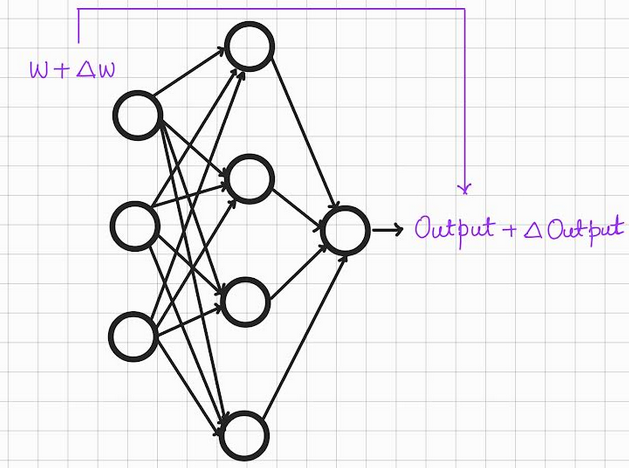
\includegraphics[width=.4\textwidth]{Figures/precepnet2.png}
\end{figure}
 
Unfortunately, a network of perceptrons doesn't have this capability. This is the reason why we use sigmoid neurons. Unlike perceptrons, the sigmoid 
neurons can take input values between $0$ and $1$. The activation function used in sigmoid neurons can be described as, 
$$\sigma(z) = \frac{1}{1 + e^{-z}}.$$
The smoothness of $\sigma$ ensures that a small change in the input causes a small change in the output. 

Figure \ref{fig:deepNN} shows an architecture of a typical (feed-forward) neural network. It consists of an input layer, multiple hidden layers and an output layer. The choice of
the number of neurons in the input and output layers is governed by the problem one is trying to solve. For example, in the case of 
hand-wriiten digit recognition, if the input image consists of data from $28 \times 28 = 784$ pixels, the input layer will have $784$ neurons. We want to classify the 
images into digits from $0$ to $9$ and therefore the output layer will have $10$ neurons. The design (number of layers and number of neurons) of hidden layers
is based on heuristics. Let us now look at a neural network (in detail) which can classify handwritten digits. 
\begin{figure}[htbp]
    \centering
    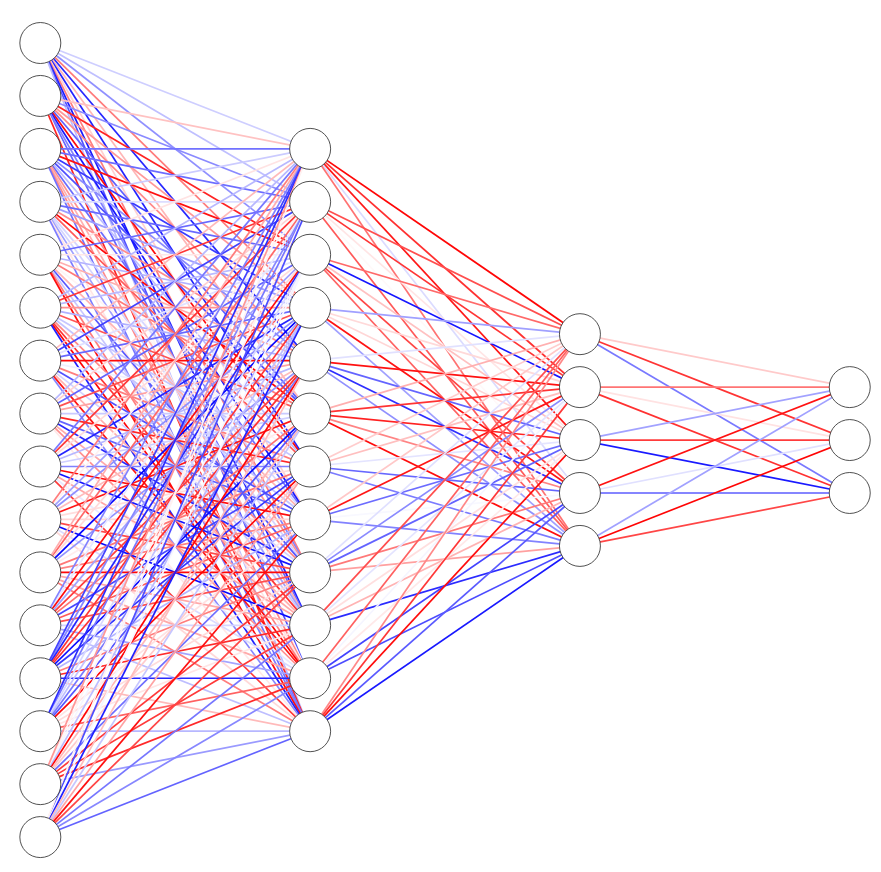
\includegraphics[width=.4\textwidth]{Figures/DeepNN.png}
    \caption{A feedforward neural network with an input layer $\in \mathbb{R}^{16}$, two hidden layers and an output layer $\in \mathbb{R}^2$.}
    \label{fig:deepNN}
\end{figure}
%%%%%%%%%%%% network to classify HD %%%%%%%%%%%%
\subsection{A network to classify handwritten digits}
We use a network consisting of an input layer $\in \mathbb{R}^{784}$, one hidden layer and an output layer $\in \mathbb{R}^{10}$ to classify handwritten
digits (see figure \ref{fig:NN_HD}). Let us try to understand how this neural network works. 
\begin{figure}[htbp]
    \centering
    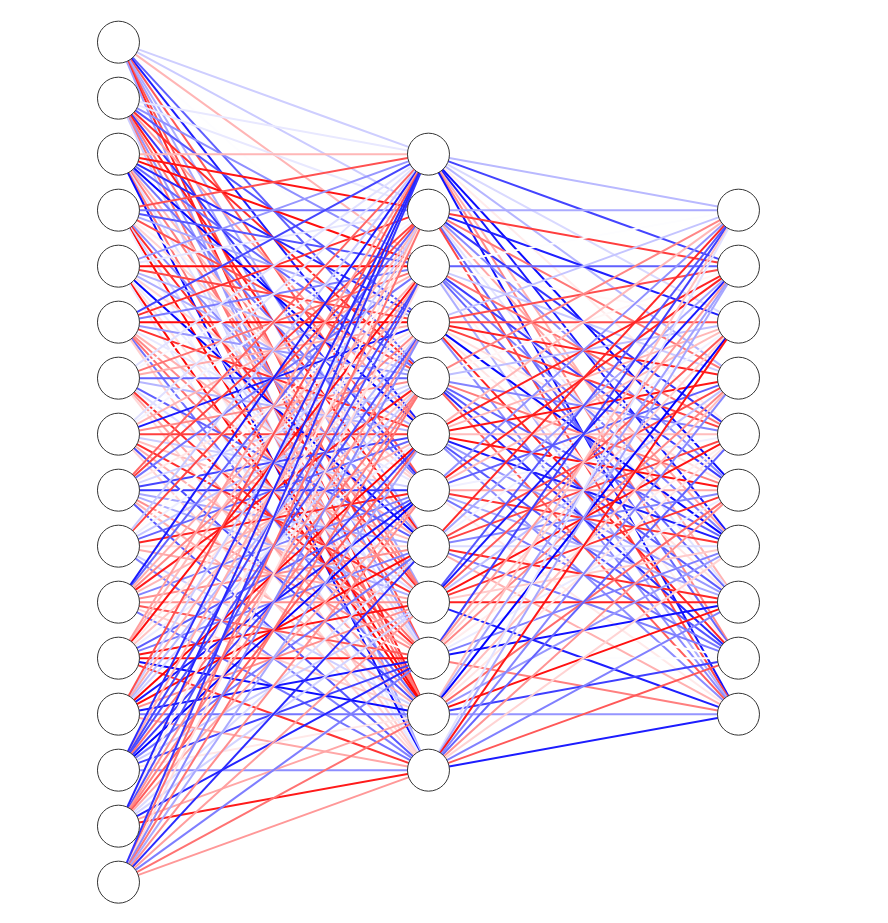
\includegraphics[width=.4\textwidth]{Figures/NN_2.png}
    \caption{A neural network to classify handwritten digits.}
    \label{fig:NN_HD}
\end{figure} 
The main feature of this network is its ability to learn from data. We use MNIST data set which consists of scanned images of handwritten digits written by $250$ people. The MNIST data
comes in two parts; a training data set containing $60000$ imgaes and a test data set containing $10000$ images. The images are in grescale and have size of $28 \times 28$ pixels.
The MNIST data, along with hand-written digits, also provide correct labels corresponding to the digits. 
\begin{figure}[htbp]
    \centering
    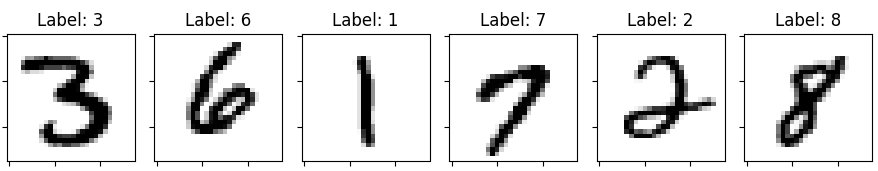
\includegraphics[width=.4\textwidth]{Figures/mnist_data_sample.png}
    \caption{A sample of training data from MNIST data set.}
    \label{fig:mnist_data}
\end{figure} 
The input $x$ to the network is a $28 \times 28 = 784$ dimensional vector and the output $a$ is a $10$ dimensional vector. In order to quantify, the 
accuracy of this network's prediction, we define a cost/loss function,
$$C(w,b) = \frac{1}{N} \sum_x {\|y(x) - a\|}^2$$
where $N$ denotes the number of training examples, $y(x)$ is the desired output (a $10$ dimensional vector) corresponding to a training example $x$, and 
$a$ is the neural network output. The idea is to find weights and biases which minimizes the difference between the desired output (labels) and the network prediction and we want this to happen for all training examples. For example, 
if an input $x$ is an image of digit $6$, we want our network's output $a$ to be as close as possible to $y(x) = (0,0,0,0,0,0,1,0,0,0)^T$. The problem of 
minimizing the loss function is an optimization problem. In the context of neural networks, the most popular methods which are used to minimize the loss function are 
inspired from the gradient descent method. 

Let us consider a simple example to understand the gradient descent method. Suppose we want to minimize a function $C(\mathbf{v})$ of two variables $v_1$ and $v_2$ (see figure \ref{fig:cost_f}).
\begin{figure}[htbp]
    \centering
    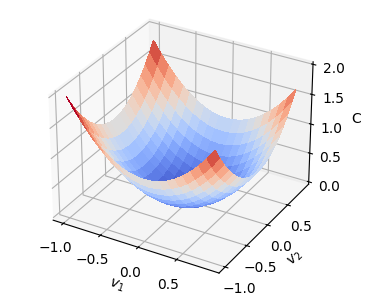
\includegraphics[width=.4\textwidth]{Figures/cost_func.png}
    \caption{A function $C$ of two variables $v_1$ and $v_2$.}
    \label{fig:cost_f}
\end{figure} 
We can use calculus to calculate the gradients of $C(\mathbf{v})$ with resprect two $v_1, v_2$ and use them to find places where $C$ is minimum. This method could work well when 
$C$ is a function of few variables but soon will turn into a nightmare when we increase the number of variables. Typically, the cost function of a neural network depends on a large number of
weights and biases; in fact the biggest neural networks consists of billions of weigths and biases. Therefore, one has to come up with cost effective 
methods of finding the minima of cost functions. Grandient descent is one such method. It is an interative method, where one starts 
with an initial guess for variables and update them over multiple iterations in such a 
way that the cost function reduces with each iteration. Consider the case of cost function $C(\mathbf{v}$). For small changes $\Delta v_1$ and  $\Delta v_2$ in variables $v_1$ and 
$v_2$ respectively, we can write the change in cost function $\Delta C$ as
\begin{equation}
    \label{eq:del_C}
    \Delta C \approx \frac{\partial C}{\partial v_1}\Delta v_1 + \frac{\partial C}{\partial v_2} \Delta v_2 = \nabla C \cdot \Delta \mathbf{v}
\end{equation}
The aim is to find suitable change $\Delta \mathbf{v}$ which leads to reduction in $C$ i.e. $\Delta C < 0$. One such choice is $\Delta \mathbf{v} = -\eta \nabla C$ provided $\eta > 0$,
$$\Delta C \approx \nabla C \cdot \eta \nabla C = \eta \|\nabla C\|^2 < 0 $$
To conclude, in the gradient descent method we start with an initial guess $\mathbf{v}$ and update it by following
 $$\mathbf{v} \rightarrow \mathbf{v}' = \mathbf{v} - \eta \nabla l$$
untill we reach the minimum of $C(\mathbf{v})$. In the context of neural networks, a gradient descent update might look like this, 
\begin{equation}
    \begin{aligned}
        w_j \rightarrow w_j' = w_j - \eta \frac{\partial C}{\partial w_j}\\
        b_k \rightarrow b_k' = b_k - \eta \frac{\partial C}{\partial b_k}.
    \end{aligned}
\end{equation}
Note that the parameter $\eta$ should be sufficiently small in order to justify the assumption in equation \eqref{eq:del_C}. 
We call this parameter the \emph{learning rate}. The use of gradient descent method might seem as a
good alternative to using analytical methods but there are still a number of challenges in applying this method. Notice that the cost function has the form
$C = \frac{1}{N} \sum_x C_x$, that is, it's an average overs costs $C_x = \|y(x) - a\|^2$ for individual training examples. In order to make an update of gradient
descent, we need to compute the gradients $\nabla C_x$ separately for each training input and then average them, $\nabla C = \frac{1}{N} \sum_x \nabla C_x$. This update can take 
extremely long time to make when the number of training inputs are very large and thus making the \emph{learning} very slow. 

We can overcome the issue of slow \emph{learning} by using a variant of gradient descent method known as \emph{stochastic gradient descent (SGD) method}. The idea is to estimate the gradient
$\nabla C$ by computing $\nabla C_x$ for a small sample of training examples and use it to make updates in weights and biases. The following steps are involved in using the stochastic gradient descent method,
\begin{enumerate}
    \item Shuffle the training inputs and divide into batches of size $m$. Each batch (we call them mini-batchs) consits of training examples say, $X_1, X_2, .....X_m$.
    \item Calculate gradients for one mini-batch: $$\frac{1}{m} \sum_{i=1}^{m} \nabla C_{X_i} \approx \frac{1}{N} \sum_x \nabla C_x = \nabla C$$
    \item Make an update in the weights and biases: 
    $$w_j \rightarrow w_j' = w_j - \frac{\eta}{m} \sum_i \frac{\partial C_{X_i}}{\partial w_j}$$
    $$b_k \rightarrow b_k' = b_k - \frac{\eta}{m} \sum_i \frac{\partial C_{X_i}}{\partial b_k}$$
    \item Pick another mini-batch from the shuffled data and repeat steps $2$ and $3$ until all training inputs are exhausted. The end of this step is referred to as an \emph{epoch} of training.
    \item Repeat steps $1$ to $5$ until the network is sufficiently trained.
\end{enumerate}
The use of SGD significantly increases the speed at which a network is trained. We may be making less accurate updates (hence the name \emph{stochastic}) in the weights and biases in comparison to 
standard gradient descent method but nevertheless the updates are faster and over multiple iterations the cost (on an average) does go down. 
\subsection{Implementation of a neural network to classify digits}
\section{Backpropagation}
Backpropagation is a fast algorithm for computing gradients. Today, it is the workhorse of learning in neural networks. It uses chain-rule from 
Calculus to compute gradients $\frac{\partial C}{\partial w_i}, \frac{\partial C}{\partial b_i}$ and in the process reveals how changing the weights and 
biases changes the overall behaviour of the network. We will first see how backpropagation works for a very simple neural network and then generalize the procdure for
big neural networks. Consider a neural network having one neuron in the input layer, two hidden layers each with one neuron and one neuron in the output layer. 
\begin{figure}[htbp]
    \centering
    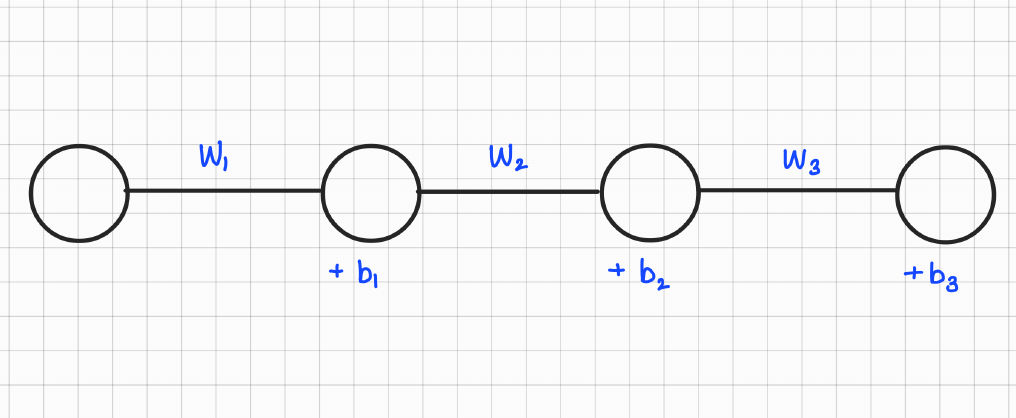
\includegraphics[width=.5\textwidth]{Figures/simpNN.png}
    \caption{A simple neural network with only neuron in each layer}
    \label{fig:sim_NN}
\end{figure} 
We can write the loss function as 
$$C = \frac{1}{N} \sum_{k=0}^{N-1} C_k.$$
Let us focus on the cost correponding to one training example,
$$C_0 = (a^{(L)} - y)^2$$ 
where $a^{(L)}$ denotes the network output and $y$ is the desired output. We label the activation/output from the last neuron with a superscript $L$, indicating which layer it's in, so the
activation of the previous neuron is $a^{(L-1)}$. We can express the last activation $a^{(L)}$ by 
$$a^{(L)} = \sigma (w^{(L)}a^{(L-1)} + b^{(L)})$$
where $w^{(L)}$ and $b^{(L)}$ denote the weight and bias of the last neuron respectively. We introduce a new variable $z$ (called weighted sum) for the input to the activation function and keep the same superscript as the activation:
$$z^{(L)} = w^{(L)} a^{(L-1)} + b^{(L)}$$
$$a^{(L)} = \sigma (z^{(L)}) $$
We first calculate $\frac{\partial C_0}{\partial w^{(L)}}$ which gives us a measure of how changes in $w^{(L)}$ affects $C_0$. We use the chain-rule from calculus and write, 
\begin{equation}
    \label{eq:sim_grad_w}
    \frac{\partial C_0}{\partial w^{(L)}} = \frac{\partial z^{(L)}}{\partial w^{(L)}} \frac{\partial a^{(L)}}{\partial z^{(L)}} \frac{\partial C_0}{\partial a^{(L)}}
\end{equation}
The terms in equation \eqref{eq:sim_grad_w} become clear if we refer to the tree of variables of the network. We can express the terms in equation \eqref{eq:sim_grad_w} by
\begin{equation*}
    \begin{aligned}
        & \frac{\partial z^{(L)}}{w^{(L)}} = a^{(L-1)} \quad \text{since} \ z^{(L)} = w^{(L)} a^{(L-1)} + b^{(L)}\\
        & \frac{\partial a^{(L)}}{\partial z^{(L)}} = \sigma'(z^{(L)}) \quad \text{since} \ a^{(L)} = \sigma (z^{(L)})\\
        & \frac{\partial C_0}{\partial a^{(L)}} = 2 (a^{(L)} - y) \quad \text{since} \ C_0 = (a^{(L)} - y)^2.
    \end{aligned}
\end{equation*}
where $\sigma'(z^{(L)})$ denotes the derivative of the activation function. This reduces equation \eqref{eq:sim_grad_w} to 
\begin{equation}
    \label{eq:del_w}
    \frac{\partial C_0}{\partial w^{(L)}} = a^{(L-1)} \cdot \sigma'(z^{(L)}) \cdot 2(a^{(L)} -y). 
\end{equation}
Next, we calculate the gradient of loss with respect to bias, $b^{(L)}$. 
$$\frac{\partial C_0}{\partial b^{(L)}} = \frac{\partial z^{(L)}}{\partial b^{(L)}} \frac{\partial a^{(L)}}{\partial z^{(L)}} \frac{\partial C_0}{\partial a^{(L)}}$$
We need to just calculate $\frac{\partial z^{(L)}}{b^{(L)}}$ in order to find $\frac{\partial C_0}{b^{(L)}}$ since the other terms are already available to us from equation \eqref{eq:sim_grad_w}. Therefore, we can write, 
\begin{equation}
    \label{del_b}
    \frac{\partial C_0}{\partial b^{(L)}} = 1 \cdot \sigma'(z^{(L)}) \cdot 2(a^{(L)} -y).
\end{equation}
At last, we calculate $\frac{\partial C_0}{\partial a^{(L-1)}}$. 
\begin{equation}
    \label{eq:del_a}
    \frac{\partial C_0}{\partial a^{(L-1)}} = \frac{\partial z^{(L)}}{a^{(L-1)}} \frac{\partial a^{(L)}}{\partial z^{(L)}} \frac{\partial C_0}{\partial a^{(L)}} = w^{(L)}\cdot\sigma'(z^{(L)}) \cdot 2(a^{(L)} -y).
\end{equation}
The procedure to obtain the cost gradient for second-last layer variables is pretty straitforward now. We just replace the superscript $L$ by $L-1$. 
\begin{equation}
    \label{eq:del_sl}
    \begin{aligned}
        &\frac{\partial C_0}{\partial w^{(L-1)}} = \frac{\partial z^{(L-1)}}{\partial w^{(L-1)}} \frac{\partial a^{(L-1)}}{\partial z^{(L-1)}} \frac{\partial C_0}{\partial a^{(L-1)}}\\
        &\frac{\partial C_0}{\partial b^{(L-1)}} = \frac{\partial z^{(L-1)}}{\partial b^{(L-1)}} \frac{\partial a^{(L-1)}}{\partial z^{(L-1)}} \frac{\partial C_0}{\partial a^{(L-1)}}
    \end{aligned}
\end{equation}
We have already calculated $\frac{\partial C_0}{\partial a^{(L-1)}}$ in the previous. For the remaining terms, we know that,
 $\frac{\partial z^{(L-1)}}{\partial w^{(L-1)}} = a^{(L-2)}$, $\frac{\partial a^{(L-1)}}{\partial z^{(L-1)}} = \sigma'(z^{(L-1)})$ and  $\frac{\partial z^{(L-1)}}{\partial b^{(L-1)}} = 1$
 thus reducing the equations \eqref{eq:del_sl} to
 \begin{equation}
    \label{eq:del_sl_f}
    \begin{aligned}
        &\frac{\partial C_0}{\partial w^{(L-1)}} =  a^{(L-2)} \cdot \sigma'(z^{(L-1)}) \cdot \frac{\partial C_0}{\partial a^{(L-1)}}\\
        &\frac{\partial C_0}{\partial b^{(L-1)}} = 1 \cdot \sigma'(z^{(L-1)}) \cdot \frac{\partial C_0}{\partial a^{(L-1)}}
    \end{aligned}
\end{equation}
\begin{figure}
\centering
    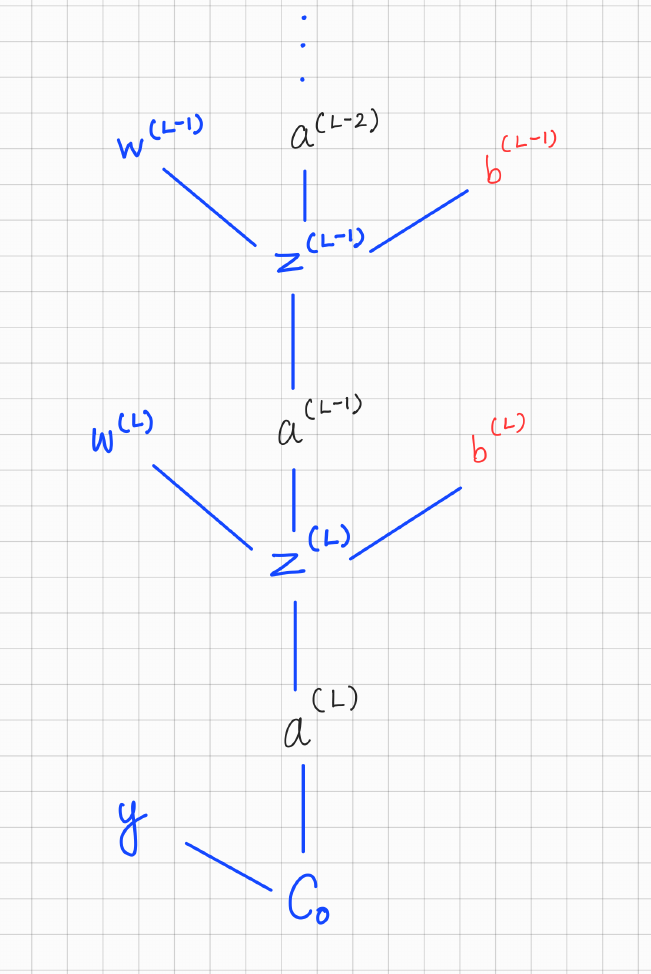
\includegraphics[width=.5\textwidth]{Figures/treeNN.png}
    \caption{This tree shows how the variables are connected in the neural network}
    \label{fig:tree_NN}
\end{figure} 
We have now finished the calculation of all gradients of the network. Although the above procedure is described for a network with only two hidden layers, 
we can easily generalize the methodology for networks with more hidden layers. In fact, the procedure is essentially the same even if we increase the number of neurons
in each layer. We demonstrate this by considering a general neural network with multiple hidden layers each having multiple neurons. 

%%%%%%%%%%% UAT %%%%%%%%%%%%%%%%%%%%%
\section{The universal approximation theorem}
Neural networks are mathematical functions. We use training data to look for suitable weights and biases
such that the neural network can map/obtain the underlying function from which the data is drawn. But, how can one
believe that a neural network have the capability of finding the underlying function. What is so special about the
neural network structure that after training it is able to give us great results on unseen data/ test data ? The answer to these
questions lies in the universal approximation theorem (UAT) proposed by George Cybenko in $1989$. 
George Cybenko gave a rigorous proof that feed-forward neural networks can approximate any continuous function defined on a compact set. To understand the 
proof of this theorem, one should be familiar with some concepts from measure theory and functional analysis. 
Let us first briefly go through those mathematical preliminaries.
\begin{itemize}
    \item Consier an $n$-dimensional unit cube, $I_n = [0,1]^n$. In the universal approximation theorem, the continuous
    functions that a neural network aims to approximate are defined on compacts sets, $I_n$ i.e. the domain of continuous
    functions is $I_n$. 
    \item Let $C(I_n)$ denote the space of continuous functions on $I_n$.
    For any function $f \in C(I_n), f : [0,1]^n \rightarrow \mathbb{R}$, one can define a suitable norm, 
    $\|f\| = \text{sup}_{x \in I_n} |f(x)|$ known as uniform/supremum norm. We can associate a dual space to $C(I_n)$ 
    defined as $C(I_n)* = \{L : C(I_n) \rightarrow \mathbb{R}\}$ where $L$ is a linear operator.
    \item UAT is defined for feed-forward neural networks having an input layer (with multiple neurons), one hidden layer and
    an output layer with only one neuron (see figure \ref{fig:ffnn_UAT}). Therefore, the functions generated by the neural network can be described as
    $$G(x) = \sum_{j=1}^{N} \alpha_j \sigma (w_j\cdot x + b_j), \quad w_j \in \mathbb{R}^n, \alpha_j, b_j \in \mathbb{R}, x \in I_n$$
    where $N$ is the number of neurons in the hidden layer. We can note that bias is not added to output from the hidden
    layer. Also the output is not passed to an activation function. We denote the set of functions of the form $G(x)$
    by $\mathcal{N}$. In the problem of hand-written digit recognition, we assumed that the activation function, $\sigma$ is logistic/sigmoid. 
    However, UAT was proved for a general class of activation functions. The actvation functions are assumed to be continuous and 
    discriminatory. 
\end{itemize} 
\begin{figure}[htbp]
    \centering
    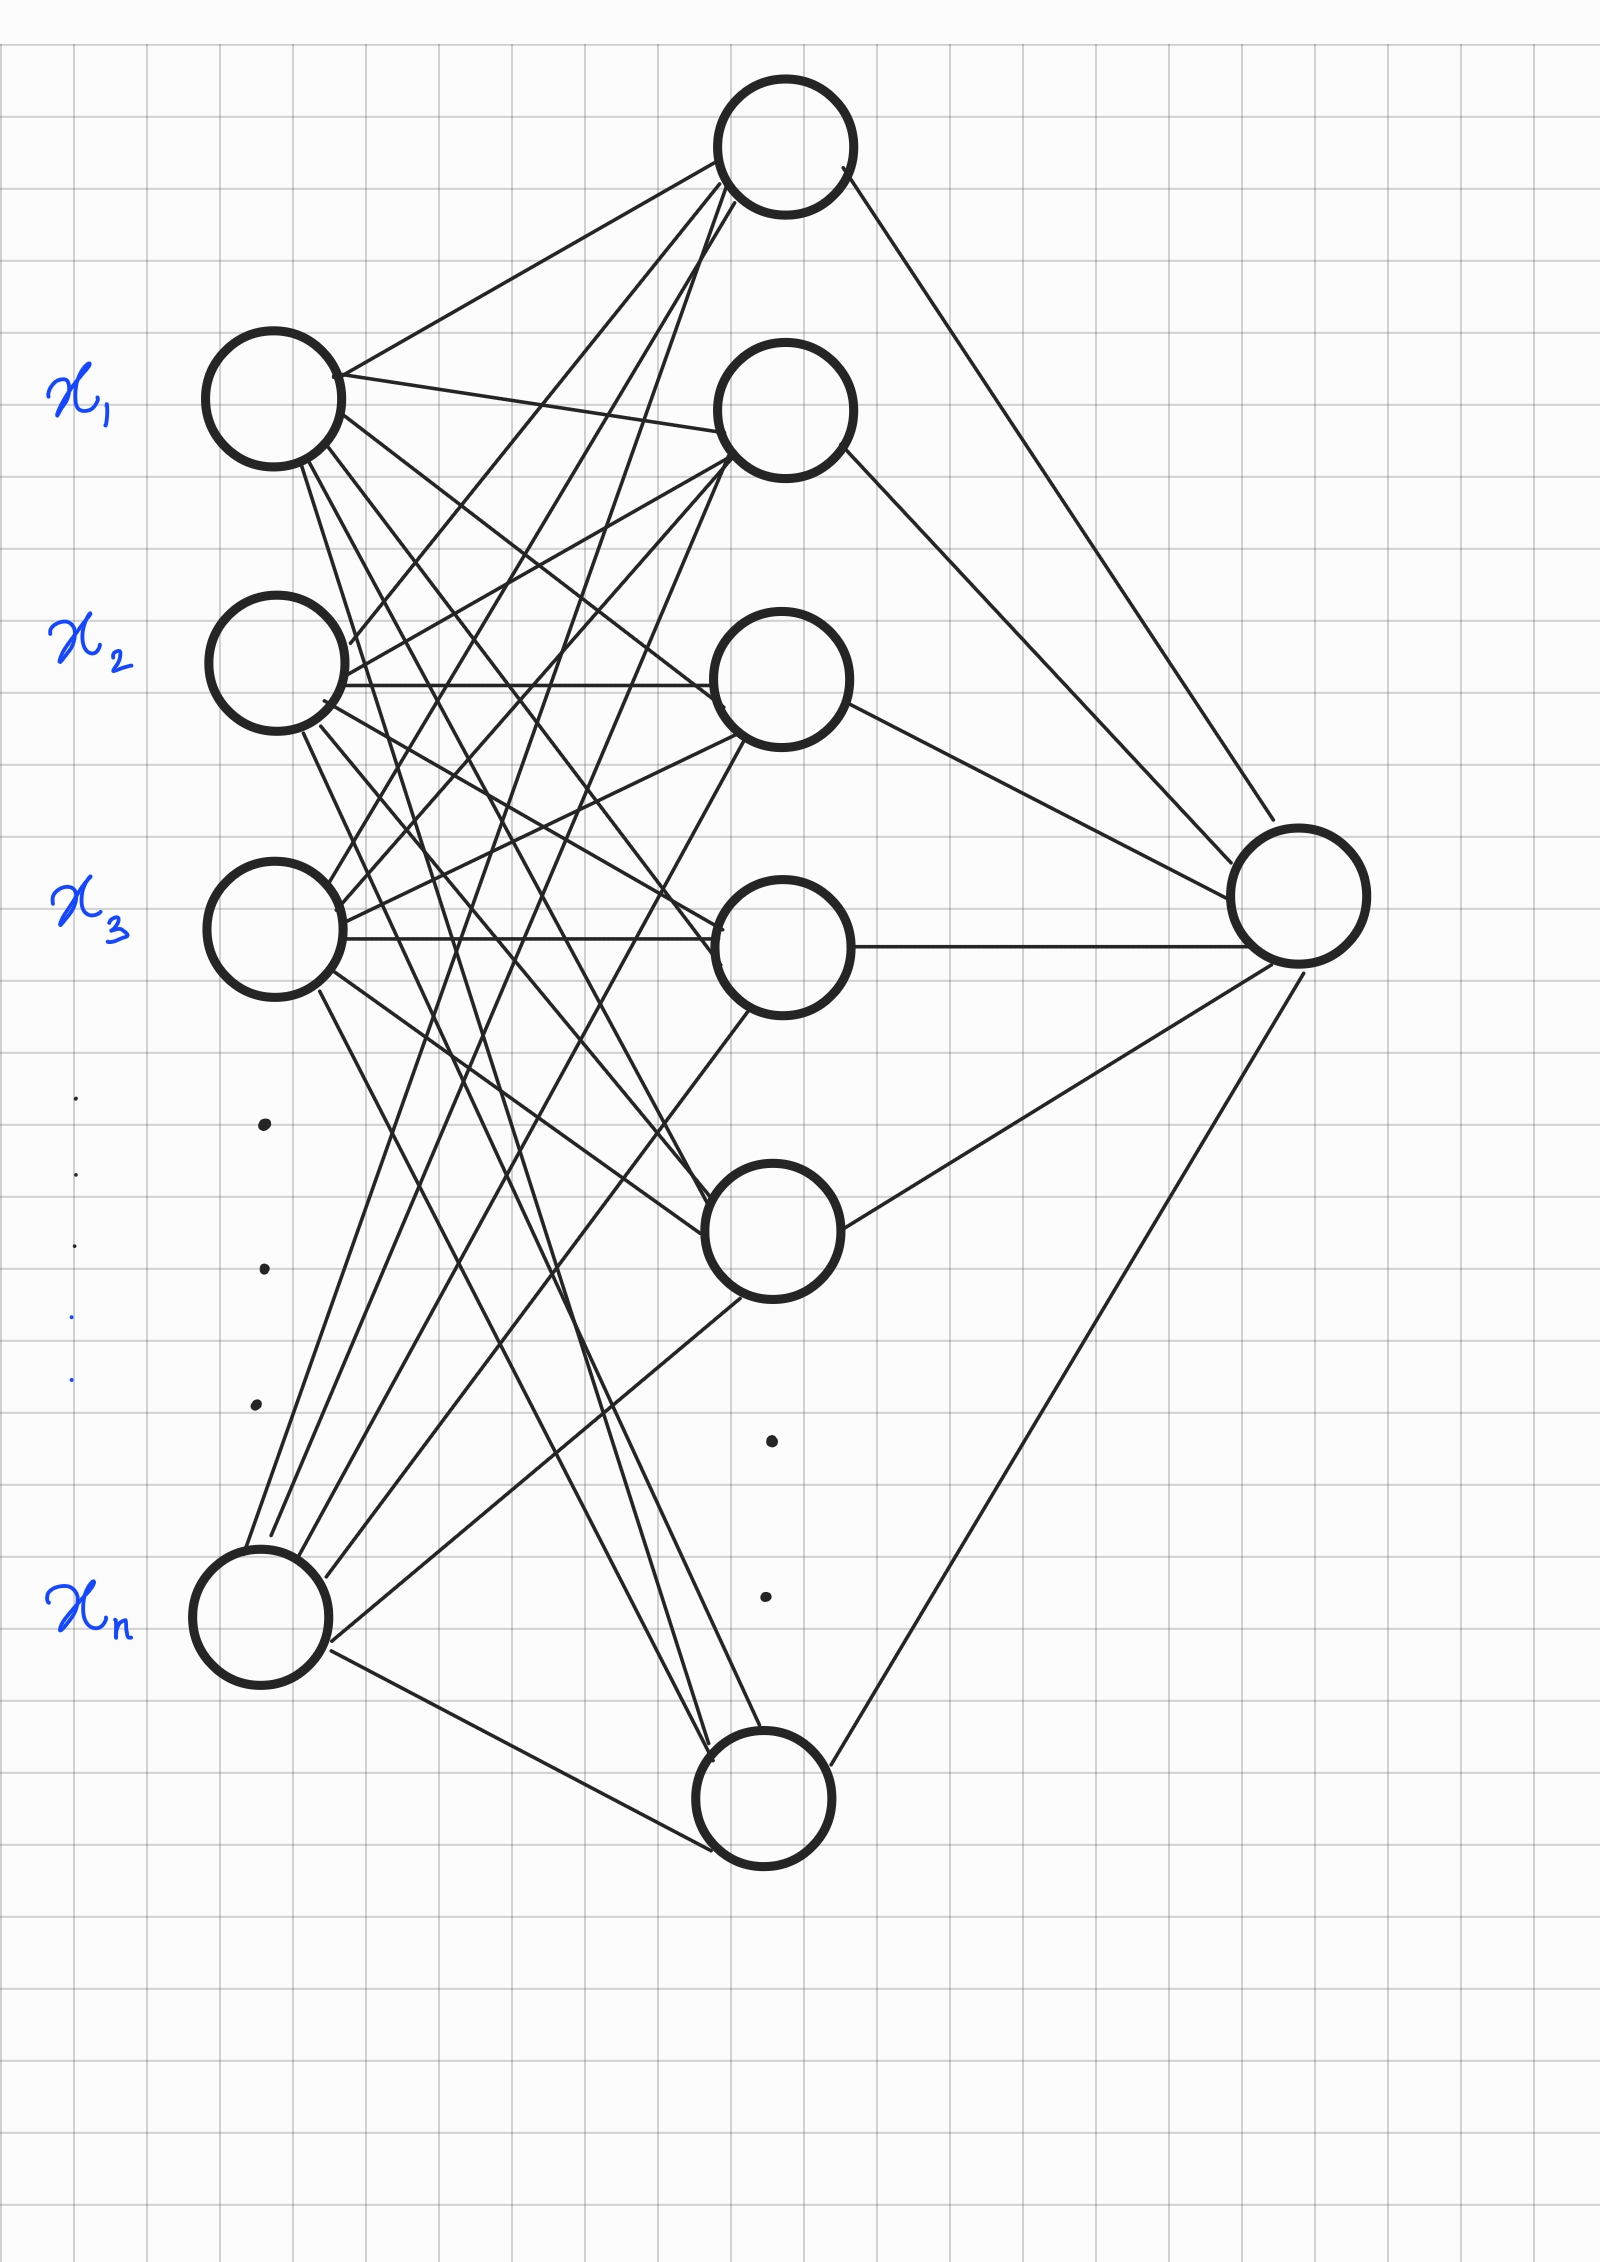
\includegraphics[width=.4\textwidth]{Figures/ffnn_UAT.jpg}
    \caption{A feed-forward neural network with an input layer (having multiple neurons), one hidden layer and an output layer (having only one neuron).}
    \label{fig:ffnn_UAT}
\end{figure}
\begin{definition}[Discriminatory function]
    We say that $\sigma$ is discriminatory if for a measure $\mu \in M(I_n)$ (where $M(I_n)$ is the space 
of finite, signed regular Borel measures on $I_n$) 
$$\int_{I_n} \sigma (\mathbf{w}\cdot\mathbf{x} + b) \ d\mu(\mathbf{x}) = 0$$
for all $\mathbf{w} \in \mathbb{R}^n$ and $b\in \mathbb{R}$ implies that $\mu = 0$.
\end{definition}
\begin{thm}[Universal approximation theorem]
    \label{thm:UAT}
    Let $\sigma$ be any continuous discriminatory function. Then the set $\mathcal{N}$ of functions of the form 
    $$G(x) = \sum_{j=1}^{N} \alpha_j \sigma (w_j\cdot x + b_j), \quad w_j \in \mathbb{R}^n, \alpha_j, b_j \in \mathbb{R}, x \in I_n$$
    are dense in $C(I_n)$. In other words, given any function $f \in C(I_n)$ and $\epsilon > 0$, there exists
    a $G(x) \in \mathcal{N}$ such that 
    $$\| G(x) - f(x)\| < \epsilon \ \text{for all} \ x \in I_n$$
\end{thm}
Before going into the proof of UAT, we will familiarize ourselfves with some key ideas from measure theory.
\begin{itemize}
    \item Our aim to measure subsets of $I_n = [0,1]^n$. A collection $\sum$ of subsets of $I_n$ is called a 
    $\sigma$-algebra if 
    \begin{enumerate}
        \item $I_n \in \sum$
        \item If $A \in \sum$, then $A^c = I_n\backslash A \in \sum$
        \item If $A_1, A_2, .....$ is a countable collection of subsets of $\sum$ then $\bigcup^\infty A_i \in \sum$.
    \end{enumerate}
    \item Borel $\sigma$-algebra on $I_n$ is the smallest $\sigma$-algebra  containing all open sets in $I_n$. Sets in Borel $\sigma$-algebra 
    are called Borel sets.
    \item A finite signed Borel measure $\mu$ on $I_n$ is a real valued  function, $\mu : \sum \rightarrow \mathbb{R}$  (where
    $\sum$ is a Borel $\sigma$-algebra defined on $I_n$) such that 
    \begin{enumerate}
        \item $\mu (\phi) = 0$
        \item $\mu (\bigcup_{i=1}^{\infty} A_i) = \sum_{i=1}^{\infty} \mu(A_i), A_i \ \text{are disjoint sets}$
        \item $\mu(A_i) < \infty$
    \end{enumerate}
    \item A Borel measure is regular if 
    \begin{align*}
        &\mu(A) = \text{sup} \{\mu(K) | K \subseteq A, K \ \text{is compact}\} \\
        &\mu(A) = \text{inf} \{\mu(U) | A \subseteq U, U \ \text{is open}\}
    \end{align*}
    In other words, what regular means is every measurable set can be approximated from above by open measurabel 
    sets and from below by compact measurable sets. 
    \item We define $M(I_n)$ as the set of all finite signed regular Borel measures on $I_n$.
\end{itemize}
The proof of UAT also uses ideas from Hahn-Banach theorem and Riesz representation theorem. These theorems 
have various equivalent versions. We now define the versions which we will refer to later. 
\begin{thm}[Riesz representation theorem]
    \label{thm:RR}
    If $K \subset \mathbb{R}^d$ is a compact set, then every linear functional $L$ defined on
    $C(K)$ can represented by a unique regular signed Borel measure $\mu \in M(K)$ in the sense that,
    $$L(f) = \int_K f \ d\mu$$
    where $f: K \rightarrow \mathbb{R}$.
\end{thm}
\begin{thm}[Hahn-Banach theorem]
    \label{thm:HB}
    Let $M$ be a linear subspace of a normed linear space $X$, and $f_0 \in X$. Then $f_0$ is 
    in the closure $\overline{M}$ of $M$ if and only if there is no bounded linear functional 
    $L$ on $X$ such that $L(f) = 0 $ for all $f\in M$ but $L(f_0) \neq 0$.
\end{thm}
We now give the proof of universal approximation theorem \ref{thm:UAT}.
\begin{proof}
   $C(I_n)$ is a vector space equipped with a supremum norm and hence is a normed vector space. It is
   clear that the set formed by functions of the form $G(x)$ is a subset of $C(I_n)$ i.e. $\mathcal{N} \subset C(I_n)$.
   We claim that $\mathcal{N}$ is also a linear subspace of $C(I_n)$. This is true due to the fact that if 
   we take two functions $G_1(x), G_2(x) \in \mathcal{N}$, we can always find a function $G_3(x) \in \mathcal{N}$ such that 
   $G_3(x) = \alpha G_1(x) + \beta G_2(x)$ for all $\alpha, \beta \in \mathbb{R}$. Our next claim is that the closure of 
   $\mathcal{N}$ is all of $C(I_n)$ i.e. $\mathcal{N}$ is dense in $C(I_n)$. We prove this by contradiction. 

   Assume that the closure of $\mathcal{N}$, $\overline{\mathcal{N}}$ is not all of $C(I_n)$ i.e. 
   $\overline{\mathcal{N}} \neq 0$. It can be proved (refer any standard functional analysis book) that $\overline{\mathcal{N}}$
   is a closed proper subspace of $C(I_n)$.  By Hahn Banach theorem \ref{thm:HB}, there exists a bounded 
   linear functional on $C(I_n)$, let's call it $L$, with the property that $L \neq 0$ but $L(\overline{\mathcal{N}}) = L(\mathcal{N}) = 0$.
   By following Riesz representation theorem \ref{thm:RR}, we can write this linear operator, $L$ as 
   $$L(h) = \int_{I_n} h(x) \ d\mu(x)$$
   for some $\mu \in M(I_n) \forall h \in C(I_n)$. Since this operator returns $0$ for all elements of $\mathcal{N}$,
   we must have for all $w \in \mathbb{R}^n, b \in \mathbb{R}$ 
   $$\int_{I_n} \sigma (w \cdot x + b) \ d\mu(x) = 0.$$
   However, we assumed that $\sigma$ is a discriminatory functions therefore this condition implies that $\mu =0$. This contradicts our initial assumption that 
   $\overline{\mathcal{N}} \neq 0$ which led to $L \neq = 0 \equiv \mu \neq 0$ via Hahn Banach theorem. Hence, the subspace $\mathcal{N}$ must be dense in $C(I_n)$. 
\end{proof}
The universal approximation theorem gives us confidence that neural networks can indeed approximate any continuous function 
provided that the activation function is continuous and discriminatory. However, it is not clear how to build activation functions which are 
discriminatory.
\begin{definition}
    \label{def:sig}
    We say that $\sigma$ is sigmoidal if 
    \begin{equation*}
        \sigma(t) \rightarrow 
         \begin{cases}
           1 &\quad \text{as} \ \ t\rightarrow +\infty\\
           0 &\quad \text{as} \ \ t\rightarrow -\infty.
         \end{cases}
    \end{equation*}
\end{definition}
\begin{lemma}
    \label{lem:sig}
    Any continuous sigmoidal function is discriminatory.
\end{lemma}
\begin{proof}
    Refer Cybenko paper.
\end{proof}
The lemma \ref{lem:sig} gives us a way to build suitable activation functions. In fact, the sigmoid/logistic function we used as an activation function
in the neural network for solving hand-written recognition problem satisfies the conditions of definition \ref{def:sig} and is therefore, discriminatory. Although 
logistic function is monotonically increasing, no monotonicity is required by definition \ref{def:sig}.
% Chapter 1
% !TeX spellcheck = en_US 
\chapter{Kernel based approximation} % Main chapter title

\label{Chapter4} % For referencing the chapter elsewhere, use \ref{Chapter1} 
\setcounter{chapter}{4}
%----------------------------------------------------------------------------------------
Kernel based methods used to be one of the main tools for machine learning up about 15 years ago, 
when neural networks became more popular.
Nowadays they are still in use due to their rich theoretical background. 
Recent interest was also spiked due to the so-called neural tangent kernel (NTK).

The first part on the following sections on kernel based approximation in mainly based on \cite{wendland2005scattered},
while the last part on the neural tangent kernel is based on recent literature \cite{jacot2018neural}.


\section{Introduction \& Motivation}

We start by discussing the following problem:

\begin{problem}
\label{prob:interpolation_problem}
Consider $\Omega \subset \R^d$ and pairwise distinct points $X_N := \{ x_i \}_{i=1}^N \subset \Omega$ and target values $\{ f_i \}_{i=1}^N \subset \R$.
Find a continuous function $s: \Omega \rightarrow \R$ that interpolates these values, i.e.\
\begin{align}
\label{eq:interpol_conditions}
s(x_i) = f_i, \qquad i=1, ..., N.
\end{align}
\end{problem}

There are two key important ingredients:
\begin{itemize}
\item Multivariate: We are not only interested in the univariate case $d=1$, but especially in the multivariate case $d>1$.
\item Meshless: The points $X_N$ may be arbitrarily unstructured and scattered, in particular we do not need any mesh.
\end{itemize}

As a first example to solve this problem, we can consider the univariate case $d=1$:
For the approximation of our problem, we pick an ansatz space $V$ with basis $\{ \phi_j \}_{j=1}^N \subset V$ and use the ansatz function
\begin{align*}
s(x) = \sum_{j=1}^N \alpha_j \phi_j(x).
\end{align*}
This ansatz function can be plugged into the system of equations from Eq.~\eqref{eq:interpol_conditions}, 
which yields the linear equation system
\begin{align}
\label{eq:lin_eq_system_general}
A_{\phi, X_N} \alpha := 
\begin{pmatrix}
\phi_1(x_1) & \phi_2(x_1) & \dots & \phi_N(x_1) \\
\phi_1(x_2) & \phi_2(x_2) & \dots & \phi_N(x_2) \\
\vdots & \vdots & \vdots & \vdots \\
\phi_1(x_N) & \phi_2(x_N) & \dots & \phi_N(x_N) \\
\end{pmatrix}
\begin{pmatrix}
\alpha_1 \\ \alpha_2 \\ \vdots \\ \alpha_N
\end{pmatrix}
=
\begin{pmatrix}
f_1 \\ f_2 \\ \vdots \\ f_N
\end{pmatrix}.
\end{align}
In order to make this more explicit, we pick the space of polynomials of degree $N-1$ as our ansatz space, 
i.e.\ $V := \pi_{N-1}(\R)$,
and as basis we choose the monomials $\{ \phi_j \}_{j=1}^N = \{ x^{j-1} \}_{j=1}^N \subset \pi_{N-1}(\R)$.
Thus the linear equation system Eq.~\eqref{eq:lin_eq_system_general} turns into
\begin{align*}
A_{\phi, X_N} \alpha := 
\begin{pmatrix}
1 & x_1 & \dots & x_1^{N-1} \\
1 & x_2 & \dots & x_2^{N-1} \\
\vdots & \vdots & \vdots & \vdots \\
1 & x_N & \dots & x_N^{N-1} \\
\end{pmatrix}
\begin{pmatrix}
\alpha_1 \\ \alpha_2 \\ \vdots \\ \alpha_N
\end{pmatrix}
=
\begin{pmatrix}
f_1 \\ f_2 \\ \vdots \\ f_N
\end{pmatrix}.
\end{align*}
The occuring matrix $A_{\phi, X_N}$ is the so-called Vandermonde matrix, and we recall that its determinant is given as
\begin{align*}
\det(A_{\phi, X_n}) = \prod_{1 \leq i < j \leq N} (x_j - x_i).
\end{align*}
Like this we can easily see, that the linear equation system Eq.~\eqref{eq:lin_eq_system_general} is uniquely solvable as soon as the points $X_N$ are pairwise distinct.

This example raises the following question:
\begin{question}
\label{question:01}
Does this procedure -- fixing a basis, and then doing interpolation with arbitrary points $X_N$ -- always work, also in higher dimensions? 
\end{question}

The answer to this question will be \textit{no}, as we will see in the Mairhuber Curtis theorem \Cref{asdf}.
In order to state and proof this theorem, we first need to introduce some mathematical notation:

\begin{definition}
	Let $\Omega \subset \R^d$ contain at least $N$ points and let $V \subseteq \mathcal{C}(\Omega)$ be an $N$-dimensional linear space. \\
	The space $V$ is called a \underline{Haar space of dimension $N$ on $\Omega$},
	if for arbitrary points $\{ x_i \} \subset \Omega$ and arbitrary values $\{ f_i \}_{i=1}^n \subset \R$ there exists a unique function $s \in V$ that satisfies 
	\begin{align*}
	s(x_i) = f_i \qquad i=1, ..., N.
	\end{align*}
\end{definition}

The polynomial spaces which we encountered before are a first example of such a Haar space:

\begin{example}
Let $\Omega = [a, b] \subset \R$ for $a < b \in \R$. 
Then $V = \pi_{N-1}(\Omega)$ (space of polynomials up to degree $N-1$ on $\Omega$) is a Haar space of dimension $N$ of $\Omega$.
\end{example}

The following proposition gives several equivalent statements on Haar spaces:

\begin{prop}
\label{prop:haar_space}
Let $\Omega \subset \R^d$ contain at least $N$ points and let $V \subseteq \mathcal{C}(\Omega)$ be an $N$-dimensional linear space. \\
Then the following statements are equivalent:
\begin{enumerate}
\item $V$ is an $N$-dimensional Haar space on $\Omega$
\item Every $v \in V \setminus \{ 0 \}$ has at most $N-1$ distinct zeros
\item For any set of pairwise distinct points $X_N \subset \Omega$ and any basis $\{ \phi_j \}_{j=1}^N$ of $V$, 
the interpolation matrix $A_{\phi, X_N}$ is invertible, i.e.\ $\det(A_{\phi, X_N}) \neq 0$.
\end{enumerate}
\end{prop}


\begin{proof}
\begin{itemize}
\item 1. $\Rightarrow$ 2.: We assume that $V$ is an $N$-dimensional Haar space on $\Omega$, 
and that there is a $v \in V \setminus \{ 0 \}$ with (at least) $N$ distinct zeros $X_N \subset \Omega$.
Additionaly we consider $u := 0$ (zero-function) and observe that $u \in V$ (as $V$ is a linear space).
Especially we have $u \neq v$.
Now, both $u$ and $v$ are distinct interpolants for the points $X_N$ with target values $f_i = 0$ for $i=1, ..., N$,
which is a contradiction to the uniqueness of the interpolant within the definition of a Haar space.
\item 2. $\Rightarrow$ 3.: We assume that there is a set of pairwise distinct points $X_N \subset \Omega$ and a basis $\{ \phi_j \}_{j=1}^N$ of $V$ such that the interpolation matrix is not invertible, i.e.\ it is singular.
Then there is a vector $\alpha \in \R^N \setminus \{ 0 \}$ such that $A_{\phi, X_N} \alpha = 0$.
As $\alpha \neq 0$, the function $v(x) := \sum_{j=1}^N \alpha_j \phi_j(x)$ is not the zero function.
However $v$ has $N$ distinct zeros (namely in the points $X_N$), which is thus a contradiction:
\begin{align*}
v(x_i) = \sum_{j=1}^N \alpha_j \phi_j(x_i) = (A_{\phi, X_n} \alpha)_i = 0 \qquad \text{for all } i=1, ..., N.
\end{align*}
\item 3. $\Leftrightarrow$ 1.: The matrix $A_{\phi, X_N}$ is invertible if and only if $A_{\phi, X_N} \alpha = b$ has a unique solution of any $b = \{f_i \}_{i=1}^N$,
which holds if and only if $\sum_{j=1}^N \alpha_j \phi_j(x_i) = f_i, i=1, ..., N$ has a unique solution $\alpha = \{ \alpha_j \}_{j=1}^N$,
which holds if and only if $s(x) := \sum_{j=1}^N \alpha_j \phi_j(x)$ is the unique interpolant.
\end{itemize}
\end{proof}

With these background knowledge on Haar spaces, we can frame \Cref{question:01} more precisely:

\begin{question}
\label{question:02}
Is there any Haar space in dimension $d>1$?
\end{question}
As announced already before, the answer to this question will be no, as established by the famous Mairhuber-Curtis theorem:


\begin{thm}[Mairhuber-Curtis]
\label{th:mairhuber_curtis}
Let $\Omega \subset \R^d$, $d>1$ be a set with nonempty interior.
Then there exists no Haar space of dimension $N>1$ on $\Omega$.
\end{thm}

\begin{proof}
For any $N$-dimensional space $V \subset \mathcal{C}(\Omega)$, we will show the existence of a set $X_N \subset \Omega$ of pairwise distinct points, 
such that the interpolation matrix has determinant zero and is thus singular, 
which is a contradiction to \Cref{prop:haar_space}:

We assume $V:= \mathrm{span} \{ \phi_1, ..., \phi_N \} \subset \mathcal{C}(\Omega)$ to be a Haar space of dimension $N > 1$ on $\Omega$.
As $\Omega$ has a nonempty interior, there exists a ball $B(x_0, \varepsilon) \subset \Omega$ for some $x_0 \in \Omega, \varepsilon > 0$.
Now we consider pairwise distinct points $X_N = \{ x_1, ..., x_N \} \subset \Omega$ with $x_1, x_2 \in B(x_0, \varepsilon)$.
As $V$ is assumed to be a Haar space, we have $\det(A_{\phi, X_N}) \neq 0$ by \Cref{prop:haar_space}. 

Now we consider continuous curves $\gamma_1, \gamma_2: [0, 1] \rightarrow B(x_0, \varepsilon) \subset \Omega$ with $\gamma_1(0) = \gamma_2(1) = x_1$, $\gamma_2(0) = \gamma_1(1) = x_2$ that do not intersect in any other points, 
that do not intersect themselves and that have no points in common with $\{x_3, ..., x_N\}$.
This is possible due to the assumption $d>1$.
Like this, $X_N(t) := \{ \gamma_1(t), \gamma_2(t), x_3, ..., x_N \}$ are pairwise distinct for any $t \in [0, 1]$.
Due to \Cref{prop:haar_space}, we have $\det(A_{\phi, X_N(1)}) \neq 0$.

Now we consider the function $D: [0, 1] \rightarrow \R, t \mapsto \det(A_{\phi, X_N(t)})$ and show that it changes sign:
As $A_{\phi, X_N} = A_{\phi, X_N(0)}$ and $A_{\phi, X_N(1)}$ only differ by a permuation of the first two rows, 
we have $D(1) = -D(0)$ and thus $D(0) D(1) < 0$.
As the function $D(t)$ is continuous, there needs to be a $\tilde{t} \in (0, 1)$ such that $D(\tilde{t}) = 0$.
This means that $X_N(\tilde{t})$ is a set of pairwise distinct points s.t.\ $A_{\phi, X_N(\tilde{t})}$ has determinant zero, which is a contradiction to \Cref{prop:haar_space}.
\end{proof}


The Mairhuber-Curtis theorem from \Cref{th:mairhuber_curtis} essentially tells us, 
that it is not possible to choose the approximation space $V$ a-priori, i.e.\ independent of the points $X_N$. 
In order to solve this issue, we will make use of kernels, which will allow us to use data-dependent approximation spaces.



\section{Kernels}

In this section, we will introduce the notion of a kernel as well as special classes of kernels 
and discuss their basic properties.
Finally we will see how interpolation can be done with kernels in a well defined way, circumventing the Mairhuber-Curtis theorem \Cref{th:mairhuber_curtis}.

We start with the basic definition of a kernel:

\begin{definition}
\label{def:kernel}
Let $\Omega$ be a nonempty set. 
\begin{itemize}
\item A \underline{real-valued kernel on $\Omega$} is a symmetric function $k: \Omega \times \Omega \rightarrow \R$.
\item A \underline{complex-valued kernel on $\Omega$} is a hermitian function $k: \Omega \times \Omega \rightarrow \R$.
\end{itemize}
\end{definition}

In the following we will mainly focus on real-valued kernels and on kernel which are defined on $\Omega \subseteq \R^d$.
However we note that kernels can be defined on very general sets that need not posses any structure, such as graphs, molecules or images.

We continue with the definition of a kernel matrix, 
which enables us to introduce the notion of positive definite (PD) and strictly positive-definite (SPD) kernels:

\begin{definition}
\label{def:positive_def_kernels}
Let $\Omega$ be a nonempty set.
\begin{itemize}
\item For any $N \in \N$ and any set of $N$ pairwise distinct points $X_N := \{ x_i \}_{i=1}^N \subset \Omega$, the \underline{kernel matrix} $A := A_{k, X_N} \in \R^{N \times N}$ is defined as $A := [k(x_i, x_j)]_{i,j=1}^N$.
\item A kernel $k$ on $\Omega$ is \underline{positive definite} (PD), if for all $N \in \N$ and all pairwise distinct points $X_N$ the kernel matrix $A$ is positive semi-definite, i.e.\
\begin{align*}
\textstyle \sum_{i,j=1}^N \alpha_i \alpha_j k(x_i, x_j) = \alpha^\top A \alpha \geq 0 \qquad \forall 0 \neq \alpha = \{ \alpha_i \}_{i=1}^N \in \R^N.
\end{align*}
\item A kernel $k$ on $\Omega$ is \underline{strictly positive definite} (SPD), if for all $N \in \N$ and all pairwise distinct points $X_N$ the kernel matrix $A$ is positive definite, i.e.\
\begin{align*}
\textstyle \sum_{i,j=1}^N \alpha_i \alpha_j k(x_i, x_j) = \alpha^\top A \alpha > 0 \qquad \forall 0 \neq \alpha = \{ \alpha_i \}_{i=1}^N \in \R^N.
\end{align*} 
\end{itemize}
\end{definition}

There is another important class of kernels, namely conditionally positive definite kernels, which are however not discussed in the following.
It is worth to note, that some literature (e.g.\ \cite{wendland2005scattered}) does not use ``\textit{strictly} positive definite'' kernels, but uses directly ``positive definite'' kernels.

In order to show why the notion of a strictly positive definite kernel is important, 
we recall the following statement from linear algebra:

\begin{prop}
\label{prop:linear_algebra}
Let $A \in \R^{N \times N}$ be a symmetric matrix. 
Then the following are equivalent:
\begin{enumerate}
\item $A$ is positive definite, i.e.\ $\alpha^\top A \alpha > 0$ for all $0 \neq \alpha \in \R^N$.
\item The eigenvalues $\{ \lambda_i \}_{i=1}^N$ of $A$ are positive
\end{enumerate}
In this case, it holds:
\begin{itemize}
\item $A$ is invertible with $\det(A) > 0$.
\end{itemize}
\end{prop}

\begin{proof}
As $A$ is symmetric, the spectral theorem gives an eigen-decomposition as $A = V\Lambda V^\top$ with $V, \Lambda \in \R^{N \times N}$, $V$ orthogonal and $\Lambda$ diagonal with the eigenvalues on its diagonal:
\begin{itemize}
\item 1. $\Rightarrow$ 2.: As $V$ is orthogonal, its columns $V_i$ form an orthonormal basis. Thus we can decompose any $0 \neq \alpha \in \R^N$ as $\alpha = \sum_{i=1}^N \beta_i V_i = V\beta$. Then we calculate:
\begin{align*}
\alpha^\top A \alpha = (\beta^\top V^\top)A(V \beta) = \beta^\top V^\top V \Lambda V^\top V \beta = \beta^\top \Lambda \beta = \sum_{i=1}^N \beta_i^2 \lambda_i.
\end{align*}
Thus $\lambda_i > 0$ implies $\alpha^\top A \alpha > 0$ for all $\alpha \neq 0$.
\item 2. $\Rightarrow$ 1.: We have $\alpha^\top A \alpha > 0$ for any $\alpha \neq 0$, thus we pick $\alpha := V_i$ (column of $V$ as specified above), and have
\begin{align*}
0 < V_i^\top A V_i \lambda_i V_i^\top V_i = \lambda_i.
\end{align*}
\end{itemize}
If all the eigenvalues are positive, also the determinant is positive due to $\det(A) = \prod_{i=1}^N \lambda_i$.
\end{proof}

\Cref{def:positive_def_kernels} in conjunction with \Cref{prop:linear_algebra} now allows us to show how strictly positive definite kernels can be used for our inteprolation problem \Cref{prob:interpolation_problem}:


\begin{thm}
Let $\Omega \subset \R^d$ and let $k$ be a SPD kernel on $\Omega$. 
For any set $\{ x_i \}_{i=1}^N \subset \Omega$ of pairwise distinct points and corresponding target values $\{ f_i \}_{i=1}^N \subset \R$,
there exists a unique kernel interpolant
\begin{align*}
s(x) := \sum_{j=1}^N \alpha_j k(x, x_j)
\end{align*}
that satisfies $s(x_i) = f_i$ for all $i=1, ..., N$. 
\end{thm}

\begin{proof}
The interpolation conditions $s(x_i) = f_i$ for all $i=1, ..., N$ yield to the linear system of equations
\begin{align}
\label{eq:lin_eq_system_kernel}
A_{k, X_N} \alpha := 
\begin{pmatrix}
k(x_1, x_1) & k(x_1, x_2) & \dots & k(x_1, x_N) \\
k(x_2, x_1) & k(x_2, x_2) & \dots & k(x_2, x_N) \\
\vdots & \vdots & \vdots & \vdots \\
k(x_N, x_1) & k(x_N, x_2) & \dots & k(x_N, x_N) \\
\end{pmatrix}
\begin{pmatrix}
\alpha_1 \\ \alpha_2 \\ \vdots \\ \alpha_N
\end{pmatrix}
=
\begin{pmatrix}
f_1 \\ f_2 \\ \vdots \\ f_N
\end{pmatrix}.
\end{align}
The matrix $A_{k, X_N}$ is exactly the kernel matrix from \Cref{def:positive_def_kernels},
and due to the assumption on the kernel to be SPD, this matrix is positive definite.
By \Cref{prop:linear_algebra} we have $\det(A_{k, X_N}) > 0$, thus this linear system of equations is uniquely solvable.
\end{proof}

As we saw that (strictly positive definite) kernels can be used for interpolation, 
we will give two examples of kernels:


\begin{example}
\label{ex:kernels}
\begin{itemize}
\item The linear kernel is defined as $k: \R^d \times \R^d: (x, z) \mapsto (x, z)_{\R^d}$. 
It simply returns the inner product of two points $x, z \in \R^d$.
It is easy to see, that the linear kernel is positive definite kernel, but not strictly positive definite.
\item The Gaussian kernel is defined as $k: \R^d \times \R^d: (x, z) \mapsto \exp(-\Vert x - z \Vert^2)$.
It makes use of the negative squared exponential of the distance between two data points, and is thus a first example of a ``radial basis function kernel''.
The Gaussian kernel can be shown to be strictly positive definite.
\end{itemize}
\end{example}



The linear kernel was a first example of a kernel, which is defined with help of a ``feature map''.
For these kind of kernels, one can directly show the positive definiteness:

\begin{thm}
\label{th:feature_map_kernel}
Let $\Omega$ be a set, $H$ a Hilbert space and $\phi: \Omega \rightarrow H$ a mapping (\underline{feature map}).
Then the kernel 
\begin{align*}
k(x, z) := (\phi(x), \phi(z))_{H}
\end{align*}
is positive definite.
\end{thm}

\begin{proof}
We verify the condition from the definition in \Cref{def:positive_def_kernels}:
\begin{align*}
\sum_{i,j=1}^N \alpha_i \alpha_j k(x_i, x_j) &= \sum_{i, j=1}^N \alpha_i \alpha_j (\phi(x_i), \phi(x_j))_H 
= (\sum_{i=1}^N \alpha_i \phi(x_i), \sum_{j=1}^N \alpha_j \phi(x_j) )_H \\
&= \left \Vert \sum_{i=1}^N \alpha_i \phi(x_i) \right \Vert_H^2 \geq 0.
\end{align*}
\end{proof}



We continue with some further elementary properties on kernels:

\begin{prop}
Let $k: \Omega \times \Omega \rightarrow \R$ be a PD kernel. Then:
\begin{itemize}
\item Non-negativity of the diagonal: 
\begin{align*}
k(x, x) \geq 0 \qquad \text{for all ~} x \in \Omega
\end{align*}
\item Cauchy-Schwarz inequality: 
\begin{align*}
k(x, z)^2 \leq k(x, x)k(z,z) \qquad \text{for all ~} x, z \in \Omega.
\end{align*}
\end{itemize}
If $k$ is SPD, then the same holds using ``$>$'' instead of ``$\geq$''.
\end{prop}

\begin{proof}
\begin{itemize}
\item We consider $N := 1$ and $X_1 = \{ x\}, \alpha = 1$. 
Then the positive definiteness implies $\alpha^\top A \alpha = k(x, x) \geq 0$.
\item We consider $N := 2$ and $X_2 = \{ x, z \}$. 
Then we have
\begin{align*}
A_{k, X_N} = \begin{pmatrix}
k(x, x) & k(x, z) \\
k(z, x) & k(z, z).
\end{pmatrix}
\end{align*}
By \Cref{prop:linear_algebra} we have $0 \leq \det(A_{k, X_N}) = k(x, x) k(z, z) - k(x, z)^2$, which can be rearranged to give the statement.
\end{itemize}
\end{proof}

The following proposition allows us to build new kernels, while maintaining their (strict) positive definiteness properties:

\begin{prop}
\label{prop:build_kernels}
Let $k_1, k_2: \Omega \times \Omega \rightarrow \R$ be PD kernels,
$f: \Omega \rightarrow \Omega$ and $g: \Omega \rightarrow \R$, $\Omega' \subset \Omega$. 
Then the following kernels are also PD (SPD):
\begin{enumerate}
\item $k: \Omega' \times \Omega' \rightarrow \R$ with $k := (k_1)|_{\Omega' \times \Omega'}$ \hfill (SPD if $k_1$ is SPD)
\item $k(x, z) := k_1(x, z) + k_2(x, z)$ \hfill (SPD if $k_1$ or $k_2$ is SPD)
\item $k(x, z) := \alpha k_1(x, z)$ for $\alpha \geq 0$ \hfill (SPD if $k_1$ is SPD and $\alpha > 0$)
\item $k(x, z) := k_1(x, z) k_2(x, z)$ \hfill (SPD if both $k_1$ and $k_2$ are SPD)
\item $k(x, z) := \exp(k_1(x, z))$ 
\item $k(x, z) := k_1(f(x), f(z)))$ \hfill (SPD if $k_1$ is SPD and $f$ is injective)
\item $k(x, z) := g(x)g(z)$
\item $k(x, z) := g(x)k_1(x, z)g(z)$ \hfill (SPD if $k_1$ is SPD and $g(x) \neq 0$)
\end{enumerate}

\end{prop}

The proofs are rather elementary and mostly directly follow from the definitions -- and are thus left as a (voluntary) homework.

Finally we will see, that the Gaussian kernel from \Cref{ex:kernels} is SPD:

\begin{prop}
The Gaussian kernel $k: \Omega \times \Omega \rightarrow \R$ for $\Omega \subset \R^d$ given as
\begin{align*}
k(x, z) = \exp(-\Vert x - z \Vert^2)
\end{align*}
is strictly positive definite.
\end{prop}

\begin{proof}
We start with the case $d=1$.
We will make use of the Fourier transform and its inverse, which are given as
\begin{align*}
\mathcal{F}[f](\omega) &:= \frac{1}{\sqrt{2\pi}} \cdot \int_{-\infty}^\infty \exp(-ix\omega) f(x) ~ \mathrm{d}x \\
\mathcal{F}^{-1}[\hat{f}](x) &:= \frac{1}{\sqrt{2\pi}} \cdot \int_{-\infty}^\infty \exp(ix\omega) \hat{f}(\omega) ~ \mathrm{d}\omega
\end{align*}
For our Gaussian kernel, we recall the following:
\begin{align*}
\mathcal{F} \left[\exp(-x^2) \right](x) &=  \frac{1}{\sqrt{2}} \cdot \exp(-\omega^2 / 4) =: \hat{\Phi}(\omega) \quad \Leftrightarrow \quad
\exp(-x^2) = \mathcal{F}^{-1} \left[\frac{1}{\sqrt{2}} \cdot \exp(-\omega^2 / 4) \right](x).
\end{align*}
With this, we can straightforward compute:
\begin{align*}
\alpha^\top A_{k, X_N} \alpha &= \sum_{j, l=1}^N \alpha_j \alpha_l k(x_j, x_l) = \sum_{j, l=1}^N \alpha_j \alpha_l e^{-(x_j - x_l)^2} \\
&= \frac{1}{\sqrt{2\pi}} \cdot \sum_{j, l=1}^N \alpha_j \alpha_l \int_{-\infty}^\infty e^{i(x_j - x_l)\omega} \hat{\Phi}(\omega) ~ \mathrm{d}\omega \\
&= \frac{1}{\sqrt{2\pi}} \cdot \int_{-\infty}^\infty \hat{\Phi}(\omega) \cdot \left| \sum_{j=1}^N \alpha_j e^{ix_j \omega} \right|^2 ~ \mathrm{d}\omega.
\end{align*}
Since $\hat{\Phi}(\omega) > 0$ and $\left| \sum_{j=1}^N \alpha_j e^{ix_j \omega} \right|^2 > 0$ a.e.\ (as $X_N$ are pairwise distinct),
we have $\alpha^\top A_{k, X_N} \alpha$.

The general case $d>0$ follows from the observation
\begin{align*}
\exp(-\Vert x - z \Vert^2) = \exp(-\sum_{i=1}^d (x^{(i)} - z^{(i)})^2) = \prod_{i=1}^d \exp(-(x^{(i)} - z^{(i)})^d)
\end{align*}
and an application of \Cref{prop:build_kernels}.

\end{proof}

It the previous proof it is worth to note, that the whole proof works as long as $\hat{\Phi}(\omega) > 0$, i.e.\ it can also be leveraged for other kernels.
This is indeed done for so-called ``translational invariant'' or ``radial basis funtion'' kernels.







\section{Reproducing kernel Hilbert spaces}

In the previous section we saw that kernel interpolation is well defined.
Now we want to consider the approximation of functions with kernel interpolation.
The properties of this approximation will for sure depend on the class of functions and on the kernel which we consider. 
In the following we will see, that there is a ``native space'' of functions, for which this works well, the so-called reproducing kernel Hilbert space (RKHS).
Within this space, we will be able to derive a  comprehensive analysis.
We start with the definition of a reproducing kernel Hilbert space:


\begin{definition}
\label{def:rkhs}
Let $\Omega$ be a nonempty set, $\mathcal{H}$ a Hilbert space of function $f: \Omega \rightarrow \R$ with inner product $(\cdot, \cdot)_{\Ha}$. \\
$\Ha$ is called a \underline{Reproducing Kernel Hilbert space} (RKHS) on $\Omega$,
if there exists a function $k: \Omega \times \Omega \rightarrow \R$ (the \underline{reproducing kernel}) such that
\begin{enumerate}
\item $k(\cdot, x) \in \Ha$ for all $x \in \Omega$
\item $(f, k(\cdot, x))_{\Ha} = f(x)$ for all $x \in \Omega, f \in \Ha$ (\underline{reproducing property})
\end{enumerate}
\end{definition}

The first point ensures, that the kernel (with fixed second argument) is a function itself within this Hilbert space of functions.
The second point, the so called reproducing property, shows that the Riesz representer of the point evaluation functional $\delta_x$ is given by $k(\cdot, x)$.

We continue with an easy example of an RKHS on $\Omega = (0, 1)$:

\begin{example}
Consider $\Omega = (0, 1)$ and the the Sobolev space $H_0^1(\Omega)$:
\begin{align*}
H_0^1(\Omega) := \{ f: [0, 1] \rightarrow \R, f \in L^2(\Omega), f' \in L^2(\Omega), f(0) = f(1) = 0 \}
\end{align*}
with inner product defined as
\begin{align*}
(f, g)_{H_0^1(\Omega)} := \int_0^1 f'(y) g'(y) ~ \mathrm{d}y
\end{align*}
Then $H_0^1(\Omega)$ is a RKHS on $\Omega$ with reproducing kernel given by
\begin{align*}
k(x, z) = \min(x, z) - xz = 
\begin{cases}
x(1-z) & \quad x < z \\
z(1-x) & \quad x \geq z.
\end{cases}
\end{align*}

As a technical note it is worth to realize, that $H_0^1(\Omega)$ consists of continuous functions due to the Sobolev embedding theorem.

Now we can quickly verify the two properties of an RKHS from \Cref{def:rkhs}: 
For the first property, we can straightforward compute $\frac{\mathrm{d}}{\mathrm{d}y} k(y, x)$ and $k(0, x)$ and $k(1, x)$ to see that $k(\cdot, x) \in H_0^1(\Omega)$.
For the second property, we calculate for any $f \in H_0^1(\Omega)$:
\begin{align*}
(f, k(\cdot, x))_{H_0^1(\Omega)} &= \int_0^1 f'(z) \frac{\mathrm{d}}{\mathrm{d}z} k(z, x) ~ \mathrm{d}z \\
&= \int_0^x f'(z) \frac{\mathrm{d}}{\mathrm{d}z} k(z, x) ~ \mathrm{d}z + \int_x^1 f'(z) \frac{\mathrm{d}}{\mathrm{d}z} k(z, x) ~ \mathrm{d}z \\
&= \int_0^x f'(z) (1-x) ~ \mathrm{d}z + \int_x^1 f'(z) (-x) ~ \mathrm{d}z \\
&= (1-x) (f(x) - f(0)) - x (f(1) - f(x)) \\
&= f(x),
\end{align*}
where we used $f(0) = f(1) = 0$ in the final step.
\end{example}

The following proposition shows that linear combinations of $k(\cdot, x_i)$ are included in the RKHS, and how to compute the inner products of such linear combinations. 
Both properties directly follow from the definition of the RKHS by leveraging the linearity of Hilbert spaces.

\begin{prop}
\label{prop:rkhs_1}
Let $\Ha$ be a RKHS on $\Omega$ with reproducing kernel $k$. 
Let $N, M \in \N$, $\alpha \in \R^N, \beta \in \R^M$ and $X_N, Z_M \subset \Omega$ and consider
\begin{align*}
f = \sum_{i=1}^N \alpha_i k(\cdot, x_i), ~ g = \sum_{j=1}^M \beta_j k(\cdot, z_j).
\end{align*}
Then it holds
\begin{enumerate}
\item $f, g \in \Ha$,
\item $(f, g)_{\Ha} = \sum_{i=1}^N \sum_{j=1}^M \alpha_i \beta_j k(x_i, z_j)$ 
\end{enumerate}
\end{prop}

\begin{proof}
\begin{enumerate}
\item By the first property within the definiton of the RKHS in \Cref{def:rkhs}, 
we have that $k(\cdot, x_i) \in \Ha$ for all $i=1, ..., N$ as well as $k(\cdot, z_j) \in \Ha$ for all $j = 1, ..., M$.
Since $H$ is a Hilbert space (by definition), it is a linear space, 
and thus also the linear combinations $f$ and $g$ are within $\Ha$.
\item To compute the inner product between $f$ and $g$, we leverage the reproducing property (second property within \Cref{def:rkhs} and make use of the linearity of the inner product:
\begin{align*}
(f, g) &= (\sum_{i=1}^N \alpha_i k(\cdot, x_i), \sum_{j=1}^M \beta_j k(\cdot, z_j))_{\Ha} \\
&= \sum_{i=1}^N \sum_{j=1}^M \alpha_i \beta_j (k(\cdot, x_i),  k(\cdot, z_j))_{\Ha} \\
&= \sum_{i=1}^N \sum_{j=1}^M \alpha_i \beta_j k(x_i, z_j).
\end{align*}
\end{enumerate}

\end{proof}

The following theorem shows that any RKHS has a kernel, that this kernel is unique, and that it is (at least) PD:


\begin{thm}
\label{thm:rkhs_1}
Let $\Ha$ be a RKHS on $\Omega$ with reproducing kernel $k$.
Then $k$ is unique and it is a PD kernel.
\end{thm}

\begin{proof}
For any $x, z \in \Omega$ we define $f := k(\cdot, x)$ and $g := k(\cdot, z)$.
From \Cref{prop:rkhs_1} we obtain $k(x, z) = (f, g)_{\Ha} = (g, f)_{\Ha} = k(z, x)$.
Thus this definition yields a valid kernel according to \Cref{def:kernel}.

We continue by proving the PDness of the kernel:
Let $X_N \subset \Omega$ be pairwise distinct and $0 \neq \alpha \in \R^N$, then we have for the kernel matrix $A$
\begin{align}
\label{eq:proof_calc_1}
\begin{aligned}
\alpha^\top A \alpha &= \sum_{i,j=1}^N \alpha_i \alpha_j k(x_i, x_j) = \left( \sum_{j=1}^N \alpha_i k(\cdot, x_i), \sum_{j=1}^N \alpha_j k(\cdot, x_j) \right)_{\Ha} \\
&= \left \Vert \sum_{i=1}^N \alpha_i k(\cdot, x_i) \right \Vert_{\Ha}^2 \geq 0.
\end{aligned}
\end{align}
Finally it is left to show that the kernel is unique.
For this assume that $k_1$ and $k_2$ are both reproducing kernels. 
By \Cref{def:rkhs} we know that $k_1(\cdot, x) \in \Ha$ as well as $k_2(\cdot, z) \in \Ha$.
By using the reproducing properties, we have
\begin{align*}
k_1(x, z) = k_1(z, x) = (k_1(\cdot, x), k_2(\cdot, z))_{\Ha} = (k_2(\cdot, z), k_1(\cdot, x))_{\Ha} = k_2(x, z),
\end{align*}
which shows that $k_1 = k_2$.
\end{proof}


Note that we cannot conclude SPD of the kernel, because within \Cref{eq:proof_calc_1} it may happen that $\{ k(\cdot, x_i) \}_{i=1}^N$ are linearly independent.
In \Cref{prop:riesz_rksh} we will see, 
that the linear independence of $\{ k(\cdot, x_i) \}_{i=1}^N$ is actually equivalent to the SPDness of the kernel.


To continue, we need to recall the Riesz representer theorem from Hilbert space theory (functional analysis).
We start with the definition of the dual space.

\begin{definition}
For a Hilbert space $\Ha$, the dual space $\Ha'$ consists of all linear and continuous functionals $\lambda: \Ha \rightarrow \R$ with norm
\begin{align*}
\Vert \lambda \Vert_{\Ha'} := \sup_{0 \neq f \in \Ha} \frac{|\lambda(f)|}{\Vert f \Vert_{\Ha}}.
\end{align*}
\end{definition}

\begin{thm}[Riesz representer theorem]
\label{thm:riesz_representer_theorem}
Let $\Ha$ be a Hilbert space and denote as $\Ha'$ its dual.
Then for all $\lambda \in \Ha'$ there exists a unique $v_\lambda \in \Ha$ (\underline{Riesz representer} of $\lambda$) such that
\begin{align*}
\lambda(f) = (v_\lambda, f)_{\Ha} \qquad \text{for all ~} f \in \Ha.
\end{align*}
Furthermore it holds $\Vert \lambda \Vert_{\Ha'} = \Vert v_\lambda \Vert_{\Ha}$.
\end{thm}

The Riesz representer theorem now allows us to further characterize RKHS:


\begin{prop}
\label{prop:riesz_rksh}
Let $\Omega$ be a nonempty set and $\Ha$ a Hilbert space of functions $f: \Omega \rightarrow \R$. 
Then
\begin{enumerate}
\item $\Ha$ is a RKHS $\Leftrightarrow$ all point evaluation functionals are continuous
\end{enumerate}
If $\Ha$ is a RKHS with kernel $k$, then
\begin{enumerate}
\setcounter{enumi}{1}
\item $k(\cdot, x)$ is the Riesz representer of the point evaluation functional $\delta_x \in \Ha'$
\item $k$ is SPD $\Leftrightarrow$ $\{ \delta_x, x \in \Omega \}$ are linearly independent
\item $|f(x)| \leq \sqrt{k(x, x)} \Vert f \Vert_{\Ha}$ for all $f \in \Ha, x \in \Omega$.
\item Convergence in $\Ha$ implies pointwise convergence
\end{enumerate}
\end{prop}


\begin{proof}
\begin{enumerate}
\item Let $\Ha$ be a RKHS, i.e.\ there exists a reproducing kernel $k$.
Then we have for the point evaluation functional $\delta_x$
\begin{align}
\label{eq:proof_calc_2}
|\delta_x(f)| = |f(x)| = |(f, k(\cdot, x))_{\Ha}|
\leq \Vert f \Vert_{\Ha} \cdot \Vert k(\cdot, x) \Vert_{\Ha}
=  \Vert f \Vert_{\Ha} \cdot \sqrt{k(x, x)},
\end{align}
i.e.\ the point evaluation functional is bounded and thus continuous.

Let $\delta_x \in \Ha'$, then 
\Cref{thm:riesz_representer_theorem} gives a Riesz representer $v_{\delta_x} \in \Ha$.
We now define $k(\cdot, x) := v_{\delta_x} \in \Ha$:
We have $k(\cdot, x) \in \Ha$ and $(f, k(\cdot, x) = (f, v_{\delta_x} = f(x)$ for all $x \in \Omega$.
Thus $\Ha$ has a reproducing kernel and thus is an RKHS.
\item The reproducing property yields $(f, k(\cdot, x)) = f(x)$ for all $x \in \Omega$. 
Furthermore $k(\cdot, x) \in \Ha$ and the Riesz representer is unique.
\item First we show that a finite set of linear functionals is linearly independent if and only if the corresponding Riesz representer are linearly independent:
\begin{itemize}
\item[] Let $\lambda_1, ..., \lambda_N$ be $N$ linearly independent functionals and $v_{\lambda_1}, ..., v_{\lambda_n}$ their corresponding Riesz representers.
We consider for any $f \in \Ha$
\begin{align*}
0 = \sum_{j=1}^N \alpha_j \lambda_j(f) = (\sum_{j=1}^N \alpha_j v_{\lambda_j},  f)_{\Ha}
\end{align*}
which can only hold for $\alpha_j = 0, j=1, ..., N$ due to the linear independence of the functionals $\lambda_1, ..., \lambda_N$.
Picking $f := \sum_{j=1}^N \alpha_j v_{\lambda_j}$ shows that also $v_{\lambda_1}, ..., v_{\lambda_N}$ are linearly independent.
\end{itemize}
In order to prove the equivalence of $k$ being SPD to $\{\delta_x, x\in\Omega\}$ being linearly independent, 
we can leverage the computation within \Cref{thm:rkhs_1},
but now we can conclude $``>''$ instead of $``\geq''$ within Eq.~\eqref{eq:proof_calc_1} due to $\{\delta_x, x\in\Omega\}$ and thus $\{ k(\cdot, x), x \in \Omega \}$ being linearly independent.
\item This was already shown in Eq.~\eqref{eq:proof_calc_2}.
\item Let $f_n \rightarrow f$ with $f, f_n \in \Ha$.
Then, by the previous point, we obtain
\begin{align*}
|(f-f_n)(x)| \leq \sqrt{k(x, x)} \cdot \Vert f - f_n \Vert_{\Ha} \rightarrow 0.
\end{align*}

\end{enumerate}
\end{proof}


In practice, we rarely start with the RKHS and think about its kernel. 
More frequently, 
we work with a kernel and are interested about its RKHS.
The following theorem gives this implication, i.e.\ how to obtain the RKHS from the kernel.

\begin{thm}[Moore-Aronszajn]
\label{th:moore_aronszajn}
Let $\Omega$ be a nonempty set and $k: \Omega \times \Omega \rightarrow \R$ a positive definite kernel.
Then there exists a unique RKHS $\ns$ with reproducing kernel $k$.
\end{thm}

\begin{proof}
The proof is constructive.
Due to \Cref{prop:rkhs_1}, we know that the finite linear combinations $\sum_{i=1}^N \alpha_i k(\cdot, x_i)$ are contained in the RKHS.
We will show, that the RKHS is given by the completion of the space given by the span of all such linear combinations:

We define
\begin{align*}
\Ha_0 := \mathrm{span} \{ k(\cdot, x), x \in \Omega \}
\end{align*}
as the space of all finite linear combinations of kernel functions with fixed second argument $x \in \Omega$.
We consider any two functions $f, g \in \Ha_0$.
By definition of $\Ha$, they can be expressed as
\begin{align}
\label{eq:representation_f_g}
\begin{aligned}
f = \sum_{i=1}^N \alpha_i k(\cdot, x_i), \\
g = \sum_{j=1}^M \beta_j k(\cdot, x_j),
\end{aligned}
\end{align}
where we can assume that $\{x_i\}_{i=1}^N \subset \Omega$ and $\{x_j\}_{i=1}^N \subset \Omega$ are each pairwise distinct.
For any such two functions $f, g$, 
we define an bilinear mapping $\mathcal{B}: \Ha_0 \times \Ha_0 \rightarrow \R$ as 
\begin{align*}
\mathcal{B}(f, g) = \mathcal{B} \left( \sum_{i=1}^N \alpha_i k(\cdot, x_i), \sum_{j=1}^M \beta_j k(\cdot, x_j) \right ) 
:= \sum_{i=1}^N \sum_{j=1}^M \alpha_i \beta_j k(x_i, x_j).
\end{align*}
We show that this mapping is well-defined, symmetric, bilinear and positive semi-definite:
\begin{itemize}
\item By definition of $f$ and $g$, it holds
\begin{align*}
\mathcal{B}(f, g) = \sum_{i=1}^N \sum_{j=1}^M \alpha_i \beta_j k(x_i, x_j) = \sum_{i=1}^N \alpha_i g(x_i) = \sum_{j=1}^M \beta_j f(x_j),
\end{align*}
i.e.\ the value of $\mathcal{B}(f, g)$ does not depend on the actual representation of $f, g$ within Eq.~\eqref{eq:representation_f_g} (which does not need to be unique),
and thus $\mathcal{B}(f, g)$ is well defined.
\item The symmetry follows directly from the definition of $\mathcal{B}$ and the symmetry of the kernel $k$.
\item The bilinearity follows as well directly from the definition of $\mathcal{B}$.
\item For the positive semi-definiteness, we compute
\begin{align*}
\mathcal{B}(f, f) = \sum_{i=1}^N \sum_{j=1}^N \alpha_i \alpha_j k(x_i, x_j) = \alpha^\top A \alpha \geq 0
\end{align*}
by the positive definiteness of the kernel $k$.
\end{itemize}
With these properties it follows that $\mathcal{B}$ is a semi inner product on $\Ha_0$, 
i.e.\ we can define $(f, g)_{\Ha_0} := \mathcal{B}(f, g)$ for $f, g \in \Ha_0$.
Especially, $\Vert f \Vert_{\Ha_0} \equiv \sqrt{(f, f)_{\Ha_0}}$ defines a semi-norm.

Now we show that $k$ is a reproducing kernel in $\Ha_0$:
Obviously we have $k(\cdot, x) \in \Ha_0$ for any $x \in \Omega$.
Furthermore we have
\begin{align*}
(f, k(\cdot, x))_{\Ha} = \sum_{i=1}^N \alpha_i k(x, x_i) = f(x),
\end{align*}
i.e.\ also the reproducing property is satisfied.
This allows us to show that the semi-inner product is actually an inner product:
Let $f \in \Ha_0$ with $\Vert f \Vert_{\Ha_0} = 0$. 
We would like to conclude $f = 0$.
To see this, we use the Cauchy-Schwarz inequality (which is applicable to semi-inner products) to estimate
\begin{align*}
|f(x)| = |(f, k(\cdot, x))_{\Ha_0}| \leq \Vert f \Vert_{\Ha_0} \cdot \Vert k(\cdot, x) \Vert_{\Ha_0},
\end{align*}
i.e.\ $\Vert f \Vert_{\Ha_0} = 0$ implies $f = 0$.

Finally we have shown that $(\Ha_0, (\cdot, \cdot)_{\Ha_0})$ is a pre-Hilbert space.
From functional analysis it is known, that pre-Hilbert spaces can be completed in an abstract way. 
We see the details in the following:
\begin{align*}
\ns := \{ f: \Omega \rightarrow \R ~ | ~ \exists \{ f_n \}_{n \in \N} \subset \Ha_0 ~ \text{Cauchy sequence s.t.~} \lim_{n\rightarrow \infty} f_n = f \}, \\
(f, g)_{\ns} := (\lim_{n \rightarrow \infty} f_n, \lim_{m \rightarrow \infty} g_m)_{\ns} = \lim_{n \rightarrow \infty} \lim_{m \rightarrow \infty} (f_n, g_m)_{\Ha_0}
\end{align*}
for $f = \lim_{n \rightarrow \infty} f_n$ and $g = \lim_{m \rightarrow \infty} g_m$.

Note that, in general, the definiton of the abstractly completed space $\ns$ is given directly by all the Cauchy sequences within $\Ha_0$.
However here we can directly identity these Cauchy sequences with a limiting function $f: \Omega \rightarrow \R$, 
because any Cauchy Sequence in $\Ha_0$ converges pointwise:
\begin{align*}
|f_n(x) - f_m(x)| \leq \Vert f_n - f_m \Vert_{\Ha_0} \sqrt{k(x, x)} \quad \text{for all~} x \in \Omega.
\end{align*}
Also observe that $\Ha_0 \subset \ns$, because for any $f \in \Ha_0$ simply consider the Cauchy sequence $\{ f \}_{i=1}^\infty$.
Next, we show that the reproducing property of $k$ within $\Ha_0$ carries over due to continuity:
\begin{align*}
f(x) = \lim_{n \rightarrow \infty} f_n(x) = \lim_{n \rightarrow \infty} (f_n, k(\cdot, x))_{Ha_0} = (\lim_{n \rightarrow \infty} f_n, k(\cdot, x))_{Ha_0} = (f, k(\cdot, x)_{\ns}.
\end{align*}
Finally we observe that $\ns$ is unique:
Assume there is another RKHS $\Ha$. 
Due to \Cref{def:rkhs} we have again $\Ha_0 \subset \Ha$, 
thus we can run the same construction and end up with $\Ha = \ns$.




\end{proof}


In \Cref{th:moore_aronszajn} we started to use the notation $\ns$ instead of $\Ha$ -- this is due to the links between a kernel and its RKHS:
\begin{itemize}
\item \Cref{thm:rkhs_1} showed that the reproducing kernel of a RKHS is unique and PD.
\item \Cref{th:moore_aronszajn} showed that every PD kernel gives rise to a unique RKHS.
\end{itemize}

In \Cref{th:feature_map_kernel} we saw, that it is possible to define kernel via a feature map. 
The following proposition shows,
that there is always a special feature map associated to a kernel:

\begin{prop}[Kernel feature map]
Let $k$ be a PD kernel on $\Omega$. 
The \underline{kernel feature map} given by $\phi: \Omega \rightarrow \ns, \phi(x) := k(\cdot, x)$ defines the kernel. 
\end{prop}

\begin{proof}
\Cref{th:moore_aronszajn} ensures the existence of $\ns$ and shows that $k(\cdot, x) \in \ns$. 
That this kernel feature map indeed defines the kernel, follows from the reproducing property:
\begin{align*}
(\phi(x), \phi(z))_{\ns} = (k(\cdot, x), k(\cdot, z))_{\ns} = k(x, z).
\end{align*}
\end{proof}



\begin{prop}
Let $k$ be a SPD kernel on $\Omega$.
If $\dim(\Omega) = \infty$, then $\dim(\ns) = \infty$.
\end{prop}


\begin{proof}
Consider $N$ pairwise distinct points $X_N \subset \Omega$.
Since $k$ is SPD, we have that $\{k(\cdot, x_j) \}_{j=1}^N$ are linearly independent by \Cref{prop:riesz_rksh}. 
Furthermore we have $\{k(\cdot, x_j) \}_{j=1}^N \subset \ns$ by definition of an RKHS in \Cref{def:rkhs}.
Thus $\mathrm{span} \{ k(\cdot, x_j), j=1, ..., N \} \subset \ns$ has dimensionality $N$.
As this holds for any $N \in \N$, we conclude $\dim(\ns) = \infty$.
\end{proof}



\section{Kernel interpololation in RKHS}

In the previous sections we saw,
that kernel interpolation is well defined and that there is a unique reproducing kernel Hilbert space of functions associated to every PD kernel.
This section focusses on analyzing properties of kernel interpolation in RKHS.
For this, we will focus on SPD kernels in the following and consider the following setting:
Given $N$ pairwise distinct points $X_N \subset \Omega$ and a function $f \in \ns$, 
we denote the kernel interpolant as $s_f$.
Then we have:


\begin{prop}
\label{prop:interpolation_projection}
Let $k$ be a SPD kernel on $\Omega$, $X_N \subset \Omega$ be $N$ pairwise distinct points and $f \in \mathcal{C}(\Omega)$. 
Consider 
\begin{align*}
V(X_N) := \mathrm{span}\{ k(\cdot, x_i), x_i \in X_N \}.
\end{align*}
\begin{enumerate}
\item $V(X_N) \subset \ns$ is an $N$-dimensional subspace
\item $s_f \in V(X_N)$
\item If $f \in \ns$, then $s_f = \Pi_{V(X_N)}(f)$ (using the orthogonal projection $\Pi_{V(X_N)}: \ns \rightarrow V(X_N)$) 
\end{enumerate}
\end{prop}

\begin{proof}
\begin{enumerate}
\item The definition of the RKHS yields that $V(X_N) \subset \ns$.
As $k$ is SPD, it follows that $V(X_N)$ is $N$-dimensional by \Cref{prop:riesz_rksh}.
\item This holds by definition of $s_f$.
\item We need to show that $f - s_f \perp V(X_N)$. 
We use that $\{ k(\cdot, x_i) \}_{i=1}^N$ is a basis of $V(X_N)$ and compute
\begin{align}
\label{eq:orthogonality_f_sf}
(f-s_f, k(\cdot, x_i))_{\ns} = (f, k(\cdot, x_i))_{\ns} - (s_f, k(\cdot, x_i))_{\ns} = f(x_i) - s_f(x_i) = 0
\end{align}
for any $i=1, ..., N$.
By linearity, this shows that $f-s_f$ is orthogonal to $V(X_N)$.
\end{enumerate}
\end{proof}

We saw that interpolation amounts to orthogonal projection.
By using properties of orthogonal projections, we can conclude the following.

\begin{coro}
\label{cor:projection_interpolant}
Let $k$ be a SPD kernel on $\Omega$, $X_N \subset \Omega$ be $N$ pairwise distinct points and $g \in \ns$.
\begin{itemize}
\item $g \in V(X_N)^\perp \Leftrightarrow g(x_i) = 0$ for all $x_i \in X_N$.
\end{itemize}
Each $f \in \ns$ can be uniquely decomposed as $f = s_f + (f-s_f)$ such that
\begin{align*}
&s_f \in V(X_N), s_f(x_i) = f(x_i) \text{~ for all\ } x_i \in X_N \\
&(f-s_f) \in V(X_N)^\perp, (f-s_f)(x_i) = 0 \text{~ for all\ } x_i \in X_N \\
&(s_f, f-s_f)_{\ns} = 0 \\
&\Vert f \Vert_{\ns}^2 = \Vert s_f \Vert_{\ns}^2 + \Vert f - s_f \Vert_{\ns}^2
\end{align*}
\end{coro}

\begin{proof}
% The statement of the bullet point is exactly the calculation from Eq.~\eqref{eq:orthogonality_f_sf}.
All the statements follow directly from properties of orthogonal projections by decomposing any $f \in \ns$ into $f = g + g^\perp$ with $g = \Pi_{V(X_N)}(f)$ and $g^\perp = \Pi_{V(X_N)^\perp}(f)$ and using $s_f = g$ and thus $g^\perp = f - s_f$. \\
For example, for the last property we have
\begin{align*}
\Vert f \Vert_{\ns}^2 &= (g + g^\perp, g + g^\perp)_{\ns} \\
&= \Vert g \Vert_{\ns}^2 + 2(g, g^\perp)_{\ns} + \Vert g^\perp \Vert_{\ns}^2 \\
&= \Vert g \Vert_{\ns}^2 + \Vert g^\perp \Vert_{\ns}^2.
\end{align*} 
\end{proof}

In the following two propositions, we will analyze two variants of our interpolation problem.
First, in \Cref{prop:best_approx_by_interpol} we will discuss what will happen, if we keep the ansatz space $V(X_N)$ but do not focus on interpolation anymore.
Second, in \Cref{prop:minimal_norm_interpol} we will discuss what will happen, if we keep the interpolation conditions, but do not focus on the ansatz space $V(X_N)$ anymore.

\begin{prop}[Best approximation by interpolation]
\label{prop:best_approx_by_interpol}
Let $k$ be a SPD kernel on $\Omega$, $X_N \subset \Omega$ be $N$ pairwise distinct points.
The kernel interpolant $s_f$ is the unique best-approximant from the space $V(X_N)$ to a function $f \in \ns$:
\begin{align*}
	\Vert f - s_f \Vert_{\ns} = \min_{s \in V(X_N)} \Vert f - s \Vert_{\ns}. 
\end{align*}
\end{prop}

\begin{proof}
This follows directly from the fact that $s_f$ is the orthogonal projection of $f$ onto $V(X_N)$, see the \Cref{prop:interpolation_projection}.
\end{proof}

\begin{prop}[Minimal norm interpolation]
\label{prop:minimal_norm_interpol}
Let $k$ be a SPD kernel on $\Omega$, $X_N \subset \Omega$ be $N$ pairwise distinct points.
Let
\begin{align*}
	S := \{ s \in \ns: s(x_i) = f(x_i), i=1, ..., N\}
\end{align*}
be the space of interpolating functions in $\ns$. 
Then it holds
\begin{align*}
\Vert s_f \Vert_{\ns} = \min_{s \in S} \Vert s \Vert_{\ns},
\end{align*}
with the minimum being unique.
\end{prop}

\begin{proof}
Apparently $s_f \in S$.
Furthermore, within $V(X_N)$, 
there is no other interpolant.
Now we show that any other interpolating function has higher norm:
Consider any $s \in S$.
By \Cref{cor:projection_interpolant} we may decompose $s = g + g^\perp$ with $g \in V(X_N)$ and $g^\perp \perp V(X_N)$.
By \Cref{cor:projection_interpolant} it furthermore follows that $g(x_i) = s(x_i) = f(x_i)$ and thus that $g = s_f$ by uniqueness of the interpolant within $V(X_N)$.
Finally we have
\begin{align*}
\Vert s \Vert_{\ns}^2 = \Vert g \Vert_{\ns}^2 + \Vert g^\perp \Vert_{\ns}^2 = \Vert s_f \Vert_{\ns}^2 + \Vert g^\perp \Vert_{\ns}^2 \geq \Vert s_f \Vert_{\ns}^2.
\end{align*}
This shows, that as soon as $s \notin V(X_N)$, we have $g^\perp \neq 0$ and thus $\Vert s \Vert_{\ns}^2 > \Vert s_f \Vert_{\ns}^2$.
\end{proof}


In the following we turn briefly to error estimates, i.e.\
ways to bound $f - s_f$.
The following proposition is very basic:

\begin{prop}[Simple bound]
Let $k$ be a SPD kernel on $\Omega$, $X \subset Y \subset \Omega$ be each pairwise distinct points and $f \in \ns$.
Let $s_{f, X}$ and $s_{f, Y}$ be the corresponding kernel interpolants.
Then it holds
\begin{align*}
V(X) &\subset V(Y) \\
\Vert s_{f, X} \Vert_{\ns} &\leq \Vert s_{f, Y} \Vert_{\ns} \leq \Vert f \Vert_{\ns} \\
\Vert f - s_{f, Y} \Vert_{\ns} &\leq \Vert f - s_{f, X} \Vert_{\ns} \leq \Vert f \Vert_{\ns}
\end{align*}
\end{prop}

\begin{proof}
As $X \subset Y$, it directly follows $V(X) \subset V(Y)$ by definition of the spaces $V(X), V(Y)$.
By \Cref{cor:projection_interpolant} we furthermore obtain $\Vert s_{f, X} \Vert_{\ns} \leq \Vert f \Vert_{\ns}$ as well as $\Vert f - s_{f, X} \Vert_{\ns} \leq \Vert f \Vert_{\ns}$.
The remaining inequalities follow likewise by \Cref{cor:projection_interpolant} by observing that the interpolant $s_{f, X}$ of $f$ in $X$ and the interpolant $s_{s_{f, Y}, X}$ of $s_{f, Y}$ in $X$ coincide due to $X \subset Y$ and $s_{f, Y}(x_i) = f(x_i)$ for all $x_i \in X$.
\end{proof}

In order to have more sophisticated error estimates, we need to introduced the power function:


\begin{definition}[Power function]
Let $s_{f, X}$ be the kernel interpolant of $f$ in $X$. 
The \underline{power function} is defined as
\begin{align}
\label{eq:power_function}
P_{X_N}(x) = \sup_{0 \neq f \in \ns} \frac{|f(x) - s_{f, X}(x)|}{\Vert f \Vert_{\ns}}
\end{align}
\end{definition}

We see, that by rearranging the definition of the power function in Eq.~\eqref{eq:power_function}, 
we immediately obtain an error bound:
\begin{align*}
|f(x) - s_f(x)| \leq P_{X_N}(x) \cdot \Vert f \Vert_{\ns}
\end{align*}
This error bound splits into the power function factor, which is independent of the function,
and the RKHS norm factor, which is independent of the points $X_N$.

However, the definition of the power function of Eq.~\eqref{eq:power_function} seems infeasbile to compute.
Therefore we will see in the following, 
how the power function can be computed in practice:

\begin{prop}
\label{prop:power_func_via_lagrange}
The power function can be computed as
\begin{align*}
P_{X_N}(x) = \sqrt{k(x, x) - \sum_{i=1}^N \sum_{j=1}^N k(x, x_i) (A^{-1})_{ij} k(x, x_j)}
\end{align*}
\end{prop}

We do not state the proof here, because it is not necessary or helpful for the following.
We stated \Cref{prop:power_func_via_lagrange} only to show that there is a computational feasible way to compute the power function:
Only the kernel and the input points $X_N$ need to be known.


%\begin{definition}[Lagrange basis]
%Let $k$ be a SPD kernel on $\Omega$, $X \subset Y \subset \Omega$ be each pairwise distinct points.
%The \underline{Lagrange basis} is defined as
%\begin{align*}
%\ell_j(x) = \sum_{i=1}^N (A^{-1})_{ij} k(x, x_i), \quad j=1, ..., N.
%\end{align*}
%
%\end{definition}
%
%\begin{prop}
%It holds $\ell_j(x_k) = \delta_{kj}$ for all $j,k=1, ..., N$.
%\end{prop}
%
%\begin{proof}
%This can be directly verified by using the definition of the Lagrange basis.
%For any $j, k = 1, ..., N$ we have
%\begin{align*}
%\ell_j(x_k) &= \sum_{i=1}^N (A^{-1})_{ij} k(x_k, x_i) = \sum_{i=1}^N (A^{-1})_{ji} A_{ik} = (A^{-1}A)_{jk} = \delta_{jk}.
%\end{align*}
%\end{proof}




\section{Translational invariant kernels and radial basis function kernels}


So far, all the results have been rather abstract.
In the following, we will briefly discuss two popular classes of kernels, namely ``translational invariant kernels'' and ``radial basis function kernels''.
We start with the definition:

\begin{definition}
A kernel $k: \R^d \times \R^d \rightarrow \R$ is called 
\begin{itemize}
\item \underline{translational invariant}, if
\begin{align*}
k(x, y) = k(x+z, y+z) \quad \text{for all\ } x, y, z \in \R^d
\end{align*}
\item \underline{radial/radially invariant}, if
\begin{align*}
k(x, y) = k(z, w)
\end{align*}
for all $x, y, z, w \in \R^d$ such that $\Vert x - z \Vert = \Vert z - w \Vert$.
\end{itemize}

\end{definition}

These kernels can be characterized in also in a different way:

\begin{prop}
A kernel $k: \R^d \times \R^d \rightarrow \R$ is 
\begin{itemize}
\item translational invariant, if and only if there exists a function $\Phi: \R^d \rightarrow \R$ such that it holds
\begin{align*}
k(x, y) = \Phi(x - y) \quad \text{for all\ } x, z \in \R^d.
\end{align*}
\item radial, if and only if there exists a function $\Phi: \R_{\geq 0} \rightarrow \R$ such that it holds
\begin{align*}
k(x, y) = \Phi(\Vert x - y \Vert) \quad \text{for all\ } x, z \in \R^d.
\end{align*}
\end{itemize}
\end{prop}

\begin{proof}
\begin{itemize}
\item Let $k(x, y) = \Phi(x-y)$. 
Then one can directly calculate
\begin{align*}
k(x + z, y + z) = \Phi(x + z - (y+z)) = \Phi(x - y) = k(x, y).
\end{align*}
Now assume that it holds
\begin{align*}
k(x, y) = k(x+z, y+z) \quad \text{for all\ } x, y, z \in \R^d.
\end{align*}
Then, for any fixed $x_0 \in \R^d$, we define $\Phi(x) = k(x_0, x_0 - x)$. 
With $z:= -x+x_0$ we can calculate
\begin{align*}
k(x, y) = k(x-x+x0, y-x+x_0) = k(x_0, x_0-(x-y)) = \Phi(x-y).
\end{align*}
It is left to show, that the definition of $\Phi$ actually does not depend on the choice of $x_0$.
Thus we consider $\tilde{x}_0 \in \R^d$ and compute
\begin{align*}
\Phi(x) = k(x_0, x_0 - x) = k(x_0 + (\tilde{x}_0 - x_0), x_0 - x + (\tilde{x}_0 - x_0)) = k(\tilde{x}_0, \tilde{x}_0 - x).
\end{align*}
This shows that the definition of $\Phi$ actually does not depend on the choice of $x_0$.
\item Let $k(x, y) = \Phi(\Vert x - y\Vert)$ and $z, w \in \R^d$ such that $\Vert x - y\Vert = \Vert z - w\Vert$. 
Then we diretly have
\begin{align*}
k(x, y) = \Phi(\Vert x - y\Vert) = \Phi(\Vert z - w\Vert) = k(z, w).
\end{align*}
Now assume that it holds $k(x, y) = k(z, w)$ for all $x, y, z, w \in \R^d$ such that $\Vert x - y \Vert = \Vert z - w \Vert$.
Then, for any fixed $x_0 \in \R^d$, we define $\Phi(r) = k(x_0, x_0 + re_1)$ with $e_1 \in \R^d$ being the first unit vector in the Euclidean system.
Consider $z := x_0$ and $w := x_0 + \Vert x - y \Vert e_1$,
which satisfy $\Vert x - y \Vert = \Vert z - w\Vert$, i.e.\
\begin{align*}
k(x, y) = k(x_0, x_0 + \Vert x - y \Vert e_1) = \Phi(\Vert x - y \Vert).
\end{align*}
As before, it is left to show that the definition of $\Phi$ actually does not depend on the choice of $x_0$ and $e_1$.
Thus consider $\tilde{x_0}, v \in \R^d$ such that $\Vert v \Vert = 1$.
We see directly
\begin{align*}
\Phi(r) \equiv k(x_0, x_0 + re_1) = k(\tilde{x}_0, \tilde{x}_0 + rv)
\end{align*}
due to $\Vert x_0 + re_1 - x_0 \Vert = r = \Vert \tilde{x}_0 + rv - \tilde{x}_0 \Vert$.
\end{itemize}

\end{proof}

We continue with some commments:
The radial kernels are frequently also called \underline{radial basis function kernels} (RBF kernels).
It is obvious, that RBF kernels are also translational invariant,
but that not every translational invariant kernel needs to be an RBF kernel.
Any RBF kernels can be tuned with help of a \underline{shape parameter} $\varepsilon > 0$ as
\begin{align*}
k(x, z) = \Phi(\varepsilon \Vert x - z \Vert).
\end{align*}
This shape parameter $\varepsilon > 0$ allows to adapt the kernel to the domain $\Omega$,
or in applications to the data $X_N$ and the corresponding target values.

In the following we will see how to deduce properties of $k$ from $\Phi$



%% \section{Basic properties and examples}
%\section{Kernels}
%
%This lecture: Definition of kernels, kernel interpolation, basic properties
%
%\begin{itemize}
%\item Definition kernel, kernel matrix, pd and spd
%\item (criteria for spd)
%\item Theorem: Kernel interpolation is well defined
%\item properties of (s)pd kernels
%\item basic operations of kernels (sum, scalar, product, exponential, ...
%\item examples of kernels: linear kernel, Gaussian kernel + Fourier + remark for RBF kernels, kernels via feature maps
%\end{itemize}


%Section 2: Basic properties and examples of kernels
%	- 2.1 Criteria for (s)pd kernels
%			Prop 2.3: i) and iii)
%	- 2.2 Properties of (s)pd kernels
%	- 2.3 Basic operations on kernels
%			o Gaussian kernel


% \section{Kernels and Hilbert spaces}
%\section{Reproducing kernel Hilbert spaces}
%
%\begin{itemize}
%\item definition RKHS + example $H_0^1$
%\item Proposition 3.5 + Characterizations
%\item Theorem Aronszajn: Existence of RKHS
%\item Feature map: Kernel feature map, other feature maps (Gaußkern, $L^2$ feature space)
%\item RKHS and smoothness, basic operations on RKHS
%\end{itemize}
%
%
%%Section 3: Kernels and Hilbert spaces
%%	- 3.1: Reproducing kernel Hilbert spaces
%%			o Definition 3.2 
%%			o Theorem 3.6
%%	- 3.2: The native space of a PD kernel
%%			o Theorem 3.10 (Aronszajn)
%%			o Prop 3.12: Kernel feature map
%%			o Prop 3.14 i)
%%			o Prop 3.15: Basic operations on kernels
%
%\section{Interpolation in RKHS}
%
%\begin{itemize}
%\item Interpolation as orthogonal projection + orthogonal decomposition
%\item Interpolation gives best approximation + minimal norm interpolation
%\item Error bounds: Definition power function, alternative form, basic properties
%\end{itemize}
%
%
%
%%Section 4: Interpolation in native spaces
%%			o Prop 4.1 (Interpolation in the native space)
%%			o Cor 4.2 (Orthogonal decomp)
%%	- 3.1: Optimality of kernel interpolation
%%			o Prop 4.3 (Interpolation gives best approximation)
%%			o Prop 4.4 (Minimal norm interpolation)
%
%
%\section{Kernels and Neural networks}
%
%\begin{itemize}
%\item Remark that we aim at providing some intuition, without discussing all mathematical details.
%It is about ongoing research
%\item (Short discussion of NNGP)
%\item Jupyter notebooks: Empirical findings: Weights change only little
%% \item Follow https://pages.cs.wisc.edu/~yliang/cs839_spring22/documents/0301-lec11-NTK-1.pdf
%\item Neural network training, solving the ODE (follow Section ``Gradient Flow'' within \url{https://rajatvd.github.io/NTK/}) + remark/discussion in which limits this hold
%\item NTK for two-layer NN
%\item Jupyter notebook: Show that training and NTK prediction actually match
%\end{itemize}
%


%----------------------------------------------------------------------------------------


% \include{Chapters/Chapter5}
\printbibliography[heading=bibintoc]
% Add more Chapters as needed...

\end{document}
